\documentclass[blue]{ludusofficial}  % Theme: blue, red, green, purple, orange, cyan
                                               % Article type: fullpaper, letter, poster, survey, shortpaper, artpaper

%% Document metadata
% \journalname{NeuroImage: Clinical}
% \journalsubtitle{International Journal of Neuroimaging in Clinical Neuroscience}
% \publicationyear{2026}
% BibLaTeX Vancouver-like numeric refs, but truncate authors to 1 + et al.
\usepackage{amsmath}
\usepackage[hyphens]{url}
\usepackage{dblfloatfix}
\usepackage{placeins}
\usepackage{afterpage}
\usepackage{lineno}
\linenumbers
\usepackage{setspace}
% NOTE: \doublespacing is applied AFTER \maketitle, not here. The class typesets the
% title, author block, abstract and keywords inside \twocolumn[...], and material in
% that optional argument is silently clipped if it exceeds one page. Double-spacing
% the 9pt abstract overflows it; the body is double-spaced below instead.
% Float placement tuning: prevent large gaps from held-back wide floats
\setcounter{topnumber}{4}
\setcounter{dbltopnumber}{4}
\setcounter{bottomnumber}{2}
\setcounter{totalnumber}{6}
\renewcommand{\topfraction}{0.95}
\renewcommand{\dbltopfraction}{0.95}
\renewcommand{\bottomfraction}{0.5}
\renewcommand{\textfraction}{0.05}
\renewcommand{\floatpagefraction}{0.8}
\renewcommand{\dblfloatpagefraction}{0.8}
%% DOI (optional - leave empty if not assigned yet)

%% Article information
\title{Longitudinal Boundary Sharpness Coefficient Slopes Do Not Improve Prediction of Alzheimer's Disease Conversion in Mild Cognitive Impairment:\\[8pt]A Landmark Survival Analysis in ADNI with External Validation}

\shorttitle{BSC Slopes and MCI-to-AD Conversion Under a Landmark Design}  % Short title for page headers
\shortauthor{Cherukuri}  % Short author names for page headers

\author{%
    \textbf{Ishaan Cherukuri}\textsuperscript{1}\textsuperscript{*}\\[0.2cm]
    \small\textsuperscript{1}Independent Researcher, USA\\
    \small Corresponding: ishaan.cherukuri@gmail.com\\[0.4cm]
    \small\textsuperscript{*}Data used in preparation of this article were obtained from the Alzheimer's Disease Neuroimaging Initiative (ADNI) database (adni.loni.usc.edu) and the Open Access Series of Imaging Studies (OASIS-3). As such, the investigators within the ADNI contributed to the design and implementation of ADNI and/or provided data but did not participate in the analysis or writing of this report. A complete listing of ADNI investigators can be found at: \href{http://adni.loni.usc.edu/wp-content/uploads/how_to_apply/ADNI_Acknowledgement_List.pdf}{adni.loni.usc.edu/how\_to\_apply/ADNI\_Acknowledgement\_List.pdf}
}

\begin{document}

%% Abstract and keywords must be defined BEFORE \maketitle
\begin{abstract}
Predicting whether someone with mild cognitive impairment (MCI) will progress to Alzheimer's disease (AD) matters for trial enrollment and for timing treatment. The Boundary Sharpness Coefficient (BSC)~\cite{olafson2021bsc} measures how sharply gray matter and white matter separate on a T1-weighted scan, and the appeal of tracking it over time is that a rate of change might carry information a single scan cannot. This study tests that idea under a design in which prediction is actually being asked of the model. Every feature comes from scans acquired while the subject was still MCI, and the survival clock starts at the last of those scans, 24 months after the MCI baseline, rather than at baseline itself. Under that landmark definition, 557 ADNI subjects (160 converters, 397 stable; median follow-up 2.5 years from the landmark, 2,005 scans inside the landmark windows) met the inclusion criteria. Six model families were compared on identical folds: penalized Cox regression, Weibull, log-normal and log-logistic accelerated failure time models, Random Survival Forest~\cite{ishwaran2008rsf}, and XGBoost with an AFT objective~\cite{chen2016xgboost}. Age, sex, education, and MMSE at the landmark reached a 5-fold cross-validated test C-index of 0.747$\pm$0.024. BSC slopes on their own reached 0.556$\pm$0.045, T1 morphometry 0.587$\pm$0.038, and adding either block to the covariates changed nothing: 0.745$\pm$0.012 for covariates plus BSC and 0.737$\pm$0.031 for covariates plus both imaging blocks. The fold-matched increment from the BSC block was $-0.000$ (95\% CI $-0.013$ to $+0.013$), the block did not improve the Cox partial likelihood ($\chi^2=5.1$, 20 df, $p=1.00$), and no individual slope separated converters from non-converters after false discovery correction. Holding the subjects, features, and pipeline fixed and changing only the follow-up definition moved BSC slope performance from 0.720 to 0.501, which locates the previously reported signal in the design rather than in the boundary. Baseline BSC magnitude also differed by scanner field strength ($d=0.30$, $p=0.003$) and tracked SNR ($r=0.22$, $p<10^{-6}$). Longitudinal BSC, measured this way, does not add prognostic information beyond routine clinical variables.
\end{abstract}



\keywords{Alzheimer's disease; mild cognitive impairment; boundary sharpness coefficient; longitudinal MRI; landmark analysis; immortal time bias; survival analysis; Cox regression; Random Survival Forest; incremental prognostic value; gray-white matter contrast; external validation; OASIS-3; MCI-to-AD conversion; ADNI}

%% Maketitle creates full-width header with abstract and keywords, then starts two-column layout
\maketitle

%% Body text is double-spaced; the front matter above keeps the class's own spacing
%% so it fits inside the single-page \twocolumn[...] block.
\doublespacing

%% From here, content is in two columns
\section{Introduction}

Alzheimer's disease (AD) already affects more than 55 million people worldwide, and projections suggest that figure could rise to 131 million by 2050~\cite{hafeez2024deep}. It remains the leading cause of dementia, accounting for roughly 60--80\% of cases, and the economic burden is staggering, now exceeding \$1 trillion globally each year. However, in practice, AD is a disease that gradually removes memory, judgment, daily independence, and eventually the basic structure of ordinary life. Biologically, this decline is related to amyloid-$\beta$ plaques, tau tangles, synaptic dysfunction, and progressive brain atrophy.

Mild Cognitive Impairment (MCI) sits in a much more uncertain space. It is not normal aging, but it is not yet dementia either. People with MCI often notice memory or thinking problems that matter, though those changes are still not severe enough to fully disrupt independent living. The difficulty is that MCI does not lead everyone down the same path. Annual conversion rates to dementia, especially AD, are often estimated around 10--15\%~\cite{li2021predicting}, yet that average hides a lot. Some individuals remain stable for years. Some even appear to improve. Others decline quickly. That uncertainty is precisely why early risk stratification matters. Treatments and interventions are most likely to help before too much irreversible damage has accumulated.

The urgency has only increased with the arrival of anti-amyloid therapies such as lecanemab~\cite{vanDyck2022lecanemab} and donanemab~\cite{sims2023donanemab}. These drugs are generally aimed at earlier stages of disease, which means clinicians and researchers need better ways to identify who is likely to progress, and when. Existing tools help, but each comes with tradeoffs. Amyloid PET can detect pathology more directly, yet it is expensive, often costing \$5,000--\$7,000 per scan, and it is not widely accessible. Cerebrospinal fluid testing provides valuable molecular information, but lumbar puncture is invasive and not always acceptable to patients. Blood-based biomarkers are increasingly promising and are beginning to enter practice, although interpretation is still not entirely straightforward because false positives and false negatives remain possible. By contrast, structural MRI is already part of standard workups for cognitive complaints, costs substantially less at roughly \$800--\$1,500, and does not require additional procedures. The catch is that conventional MRI markers, especially when measured at only one time point, have often been disappointing for prediction~\cite{baytas2024predicting}.

\subsection{Prior Work and the Gaps This Study Addresses}

Prediction of MCI-to-AD progression is a mature literature, and two systematic reviews map it well enough to make individual comparisons meaningful. Ansart et al.~\cite{ansart2021predicting} screened 234 studies and extracted results from 111 of them. Grueso and Viejo-Sobera~\cite{grueso2021machine} reviewed 116 machine learning studies over a similar period. Read together, they support four conclusions that shaped the design used here.

The first is that cognitive testing is a strong and cheap predictor. In the Ansart review, models using cognitive scores alone reached a mean AUC near 0.78, statistically indistinguishable from models using MRI alone, and combinations of cognition with imaging performed best. A new imaging marker therefore has to be judged against cognition and demographics, not against an empty model. Studies that omit age, sex, education, and a baseline cognitive score cannot say whether their marker adds anything, and a substantial fraction of the reviewed literature omits them.

The second is that reported performance depends heavily on design choices that have nothing to do with the biomarker. Ansart et al. found that studies using a single train-test split reported higher performance than those using cross-validation, that small samples inflate results, and that the definition of the prediction window varies widely across papers. Grueso and Viejo-Sobera reach a similar conclusion and note that few studies report an external test at all.

The third gap concerns time. Most of this literature treats conversion as a binary label within a fixed horizon, which discards censoring and forces an arbitrary cutoff. Time-to-event formulations handle both properly and are increasingly used. Li et al.~\cite{li2017prediction} fit joint models linking longitudinal cognitive and imaging trajectories to conversion time in ADNI. Zhang et al.~\cite{zhang2024interval} point out that conversion is interval-censored, since it is only ever observed between two clinic visits, and compare interval-censored models on that basis. Da et al.~\cite{da2014integration} quantify the relative value of atrophy patterns, cognition, APOE, and CSF within a single survival framework, and find that no imaging marker displaces cognition. The present study sits in that tradition and adopts its accounting: the comparator is a clinical model, and the question is incremental value.

The fourth gap is where this study originally went wrong, and it is worth stating plainly because it motivates the redesign. In a longitudinal design the features are computed from a series of scans, but the survival clock has to start after the last scan that contributed to those features. If it starts earlier, subjects are guaranteed to be event-free over the period in which their own predictors were measured, which is guarantee-time or immortal time bias~\cite{anderson1983analysis,giobbie2013guarantee}. Worse, scans acquired after a dementia diagnosis can end up inside the feature window, so the model is shown the disease it is asked to forecast. The remedy is a landmark design~\cite{anderson1983analysis}: fix a landmark time, use only data available at that point, exclude subjects who have already converted, and follow the rest forward. The analysis below is built that way, and the difference it makes is one of the main results.

A fifth issue is generalization. Nearly all reported figures come from one cohort, usually ADNI, assessed by cross-validation. Cross-validation protects against fitting particular subjects too closely. It does nothing about fitting a cohort's scanners, protocols, recruitment habits, or follow-up schedule. This study therefore keeps the transfer test to OASIS-3 as a result in its own right.

Within that landscape, work on individual markers is easy to overrate. Li et al.~\cite{li2021predicting} reported an AUC of 83\% by combining genetic data, gene expression, and neuroimaging, though such pipelines demand blood collection and specialized assays. Studies mining electronic health records report accuracies around 72\% several years before diagnosis~\cite{north2025breakthroughs}, but they capture downstream clinical traces rather than brain tissue. Hafeez et al.~\cite{hafeez2024deep} classified established AD with 96\% accuracy from imaging snapshots while reaching 84\% for conversion, which is a useful reminder that recognizing disease and forecasting it are different problems.

\subsection{The Boundary Sharpness Coefficient}

The Boundary Sharpness Coefficient (BSC) measures how sharply gray matter and white matter are separated on structural MRI. In a healthy brain, the transition between the cortical gray matter and the underlying white matter is usually fairly crisp on a T1-weighted scan. Gray matter tends to appear darker, while white matter is brighter because of its myelin-rich composition. When disease-related processes disrupt that organization, the interface can become less distinct.

BSC is therefore different from more familiar measures such as regional volume or cortical thickness. Those metrics tell us how much tissue remains. BSC, instead, captures a boundary property. It is not a direct microscope-like readout of microstructure, and it would be overstating things to claim otherwise. Still, it may reflect biologically meaningful changes at the gray-white matter interface before more obvious atrophy becomes visible. In that sense, it occupies an interesting middle ground between gross anatomy and finer tissue organization.

\subsubsection{Relation to Gray-White Intensity Contrast and to Junction Blurring}

BSC is not the first attempt to quantify this interface, and its relationship to two older measures should be stated before any claim of novelty. Salat et al.~\cite{salat2009age} measured gray-white matter intensity contrast as the normalized difference between sampled gray and white matter signal on either side of the surface. That measure declines with age, changes independently of cortical thickness, and is now a standard descriptor of the interface. Huppertz et al.~\cite{huppertz2005enhanced} approached the same anatomy from the other direction in epilepsy, building a junction image that flags voxels with abnormally blurred gray-white transitions to localize focal cortical dysplasia.

BSC differs from both in what it measures at a voxel. Intensity contrast is a difference of levels, sampled at fixed distances from the surface. Junction images threshold a blurring index against a normal template. BSC is a projected gradient: it takes the spatial derivative of intensity and keeps the component aligned with the tissue-probability normal, so it describes how quickly signal changes across the interface rather than how far apart the two tissues sit. In a noise-free image with a step edge these are monotonically related, and in real data they are correlated but not equivalent, since a boundary can lose contrast while staying geometrically crisp, or blur while retaining the same endpoint intensities. The practical consequence is that BSC inherits most of the confounds of intensity contrast while adding those of a derivative operator.

Those confounds define the failure modes and are treated as testable in this study rather than as caveats. A gradient magnitude scales with image contrast, so any influence on tissue contrast propagates into BSC. Field strength is the obvious one, since 1.5T and 3T acquisitions differ in T1 contrast and in noise. Motion blurs edges and lowers measured sharpness without any tissue change. Bias field, interpolation during resampling, and the smoothing width used for the derivative all set a floor on measurable sharpness. Segmentation error moves the boundary band itself, so the same voxels are not necessarily sampled across visits. In a longitudinal design any of these can drift with time and masquerade as a slope, particularly when a subject changes scanner mid-study. Section~\ref{sec:acquisition} reports what these dependencies look like in this cohort.

Several pathological processes in AD could plausibly blur this boundary. Amyloid and tau pathology disrupt neuronal integrity. Synaptic loss changes cortical organization. Inflammation alters tissue composition. Myelin degeneration affects white matter signal properties. None of those processes maps one-to-one onto BSC, but together they provide a reasonable biological basis for why boundary sharpness might deteriorate as disease advances.

BSC computation in this study followed a multi-step pipeline (Figure~\ref{fig:pipeline}). First, Atropos k-means clustering~\cite{avants2011atropos} assigned each voxel a probability of belonging to gray matter, white matter, or cerebrospinal fluid. Next, boundary voxels were defined as those where gray matter probability fell between 0.4 and 0.6, which captures a transition band rather than forcing the analysis onto an unstable single-voxel contour. Gradient filters then measured how rapidly MRI intensity changed across that boundary, and the gradient was projected along the direction perpendicular to the interface. For each boundary voxel $\mathbf{x}$, the directional BSC was computed as follows:

\begin{figure*}[!htbp]
\centering
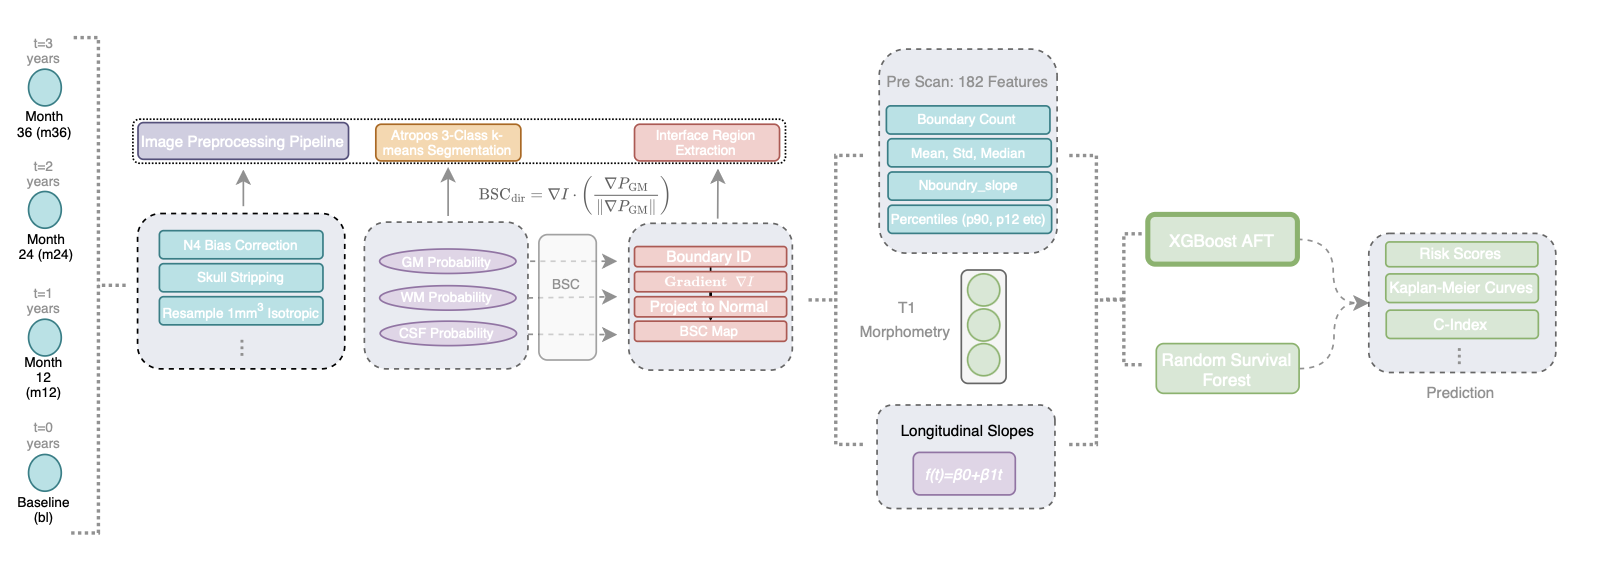
\includegraphics[width=0.95\textwidth]{Trillium/arch.png}
\caption{Complete BSC slope-based MCI-to-AD conversion prediction pipeline. Longitudinal T1-weighted MRI scans undergo preprocessing (N4 bias correction, skull stripping, resampling), Atropos segmentation to derive GM/WM probability maps, and BSC computation at the gray-white matter boundary. Per-scan features (33 total) are extracted from each time point, then organized into per-subject longitudinal sequences. Linear regression across the time points inside the landmark window yields slope-based features per subject capturing annual rates of boundary degradation. The top 20 most variable slopes are selected inside each training fold and combined with 60 T1 morphometry features and four clinical covariates, giving an 84-column matrix that is passed to six model families. Only scans acquired while the subject was still MCI enter this pipeline, and survival time is measured from the landmark onwards. The figure shows the pipeline as run for this revision; the schematic layout is unchanged from the submitted version, in which features were drawn from every available scan.}
\label{fig:pipeline}
\end{figure*}

\begin{equation}
    \text{BSC}_{\text{dir}}(\mathbf{x}) = \nabla I(\mathbf{x}) \cdot \frac{\nabla P_{GM}(\mathbf{x})}{\|\nabla P_{GM}(\mathbf{x})\|}
\end{equation}

Here, $I(\mathbf{x})$ denotes MRI intensity at voxel $\mathbf{x}$ and $P_{GM}$ is the gray matter probability map. The term $\nabla I$ measures how quickly intensity changes in space, while the dot product isolates the component aligned with the boundary normal. Positive values indicate the expected increase in intensity when moving from gray matter toward white matter. Negative values usually reflect artifacts or local reversals.

The final output is a three-dimensional map in which each boundary voxel is assigned a sharpness value. Those voxel-level measurements are then summarized using means, medians, standard deviations, and percentiles so they can be used in downstream statistical models.

\subsection{From Static Measures to Temporal Slopes}

The weakness of single-timepoint biomarkers is not merely that people have different head sizes or different baseline anatomy. Those issues can often be normalized. The deeper problem is that a cross-sectional scan mixes together many influences that have accumulated across a lifetime. Two people can show the same hippocampal volume, for instance, while meaning very different things biologically. One may simply have had a smaller hippocampus for years. The other may be in the middle of active neurodegeneration. A single snapshot cannot really distinguish those scenarios.

Cognitive reserve complicates the picture even more. Some individuals tolerate substantial pathology before symptoms become obvious. Education, occupational complexity, social engagement, and lifelong learning may all contribute to that resilience. So a person can look relatively intact on standard cognitive tests while disease processes are already advancing beneath the surface.

That is why rates of change are so appealing. A declining trajectory can reveal ongoing pathology in a way that baseline values often cannot. The working hypothesis here is that \textbf{longitudinal BSC slopes}, meaning annualized rates of change in boundary sharpness features, capture progression dynamics that are largely invisible in a baseline scan. Someone whose BSC is deteriorating quickly may face a very different future from someone who starts at a similar level but remains stable over time. That reasoning is sound, and it is worth testing carefully, because a trajectory measured over a window that overlaps the outcome will look predictive whether or not the reasoning holds. The results below do not support the hypothesis once that overlap is removed.

\subsection{Study Objectives}

This study was guided by six aims:

\begin{enumerate}
    \item Rebuild the cohort under a landmark design so that every feature is derived from scans acquired while the subject was still MCI, with follow-up starting at the last such scan
    \item Compute longitudinal BSC slopes and matched T1 morphometry trajectories within that pre-conversion window
    \item Establish a clinical reference model from age, sex, education, and MMSE at the landmark
    \item Test whether BSC slopes add discrimination to that reference model, and to established longitudinal MRI measures, using fold-matched comparisons across six model families
    \item Quantify how much of the previously reported performance is attributable to the follow-up definition alone
    \item Characterize the dependence of BSC on acquisition factors, and test whether the fitted model transfers to an independent OASIS-3 cohort
\end{enumerate}

\section{Materials and Methods}

\subsection{Dataset and Study Population}

Primary data were obtained from the Alzheimer's Disease Neuroimaging Initiative (ADNI) database (\texttt{adni.loni.usc.edu})~\cite{weiner2010adni,petersen2010adni}. ADNI began in 2003 as a large public-private effort led by Michael W. Weiner, MD, with the goal of determining whether serial MRI, PET, fluid biomarkers, and cognitive testing could track the progression of MCI and early AD. Over time, ADNI has become one of the most widely used open neuroimaging resources in the field. Its strengths are fairly clear: standardized protocols, repeated follow-up, and broad data sharing. At the same time, like many research cohorts, it is not a perfect mirror of routine clinical populations, which matters when thinking about generalizability.

Scans were drawn from the BIDS-converted ADNI-1, ADNI-GO/2, ADNI-3, and ADNI-4 releases and joined against the ADNIMERGE2 DXSUM table for per-visit diagnosis and visit dates. BIDS-converted files carry no absolute acquisition date, so dates were reconstructed as the subject's earliest DXSUM visit date plus the month offset parsed from the session label, with diagnosis assigned by nearest-date match against that subject's visit history. Sessions with no parseable offset were skipped.

\subsubsection{Landmark Design and Definition of Follow-up}
\label{sec:landmark}

The unit of analysis is a subject observed at a landmark time, not a subject observed from baseline. The landmark was set at 24 months after the first MCI scan, with a 90-day grace window so that a visit acquired slightly late still counts toward its nominal timepoint. Three rules follow from that choice, and together they define the cohort.

Only scans acquired on or before the landmark contribute to any feature. Nothing acquired afterwards enters the model, which rules out the case where a scan taken at or after the dementia visit is used to predict that same dementia visit.

Subjects who had already converted at or before the landmark were excluded rather than treated as events. A subject who is already demented at the landmark is not at risk of converting after it, and including them turns prediction into detection.

Follow-up time runs from the landmark date to the first clinical visit at which the diagnosis reached dementia, or to the last available clinical visit for subjects who did not convert. Conversion and censoring dates come from the ADNIMERGE2 DXSUM clinical record rather than from the diagnosis attached to a scan. This matters more than it sounds: if censoring is taken from the last MRI, then every non-converter has zero follow-up after their own last scan, and no landmark analysis is possible at all. Because a diagnosis is only ever recorded at a visit, the true conversion time lies somewhere between the last MCI visit and the first dementia visit, so these times are interval-censored and are treated here as right-censored at the first dementia visit, which is the conventional approximation~\cite{zhang2024interval}.

The choice of 24 months trades cohort size against the number of scans available for a slope. A 12-month landmark leaves most subjects with only two scans, which makes a slope a difference and an $R^2$ undefined. A 36-month landmark loses more converters to the pre-landmark exclusion. At 24 months, subjects contribute a mean of 3.6 scans over a mean window of 1.65 years. A subject-specific landmark placed at each subject's own last pre-conversion scan is reported as a sensitivity analysis in Section~\ref{sec:sensitivity}.

\subsubsection{Inclusion Criteria}

Subjects were included if they met five criteria: MCI at the first available scan, at least two T1-weighted scans on distinct dates within the landmark window, per-visit diagnosis available from DXSUM, non-zero follow-up after the landmark, and successful completion of the segmentation and BSC pipeline at every retained time point.

Of the 1,604 subjects with processed scans, 421 were not MCI at their first scan, 219 had already converted at or before the landmark, 249 had fewer than two scans inside the window, and 158 had no clinical follow-up after the landmark. That leaves \textbf{557 subjects} with \textbf{160 converters} and \textbf{397 stable subjects}. Median follow-up from the landmark was 2.51 years (mean 3.66), and median time to conversion among converters was 1.77 years. For comparison, the same pipeline run under the submitted design, with the clock starting at the baseline scan and every scan contributing features, yields 657 subjects, which is the cohort reported previously.

\afterpage{%
\begin{table*}[!t]
\centering
\caption{Demographic and clinical characteristics of the study cohort}
\label{tab:demographics}
\begin{tabular}{lccc}
\hline
\textbf{Characteristic} & \textbf{All} & \textbf{Converters} & \textbf{Stable} \\
 & (N=557) & (N=160) & (N=397) \\
\hline
Age at landmark (years) & 74.8$\pm$7.4 & 76.6$\pm$6.8 & 74.0$\pm$7.5 \\
Female, n (\%) & 234 (42.0) & 66 (41.2) & 168 (42.3) \\
Education (years) & 16.2$\pm$2.7 & 16.1$\pm$2.7 & 16.2$\pm$2.7 \\
MMSE at landmark & 27.6$\pm$2.5 & 26.3$\pm$2.7 & 28.1$\pm$2.2 \\
Scans in landmark window & 3.60$\pm$0.82 & 3.58$\pm$0.89 & 3.61$\pm$0.80 \\
Window span (years) & 1.65$\pm$0.37 & 1.66$\pm$0.38 & 1.65$\pm$0.37 \\
Follow-up from landmark (years) & 3.66$\pm$3.42 & 2.71$\pm$2.62 & 4.05$\pm$3.63 \\
\hline
\multicolumn{4}{p{0.62\textwidth}}{\footnotesize Values are mean$\pm$SD unless stated. Follow-up is measured from the landmark, 24 months after the first MCI scan, not from that first scan. MMSE was taken from the clinical visit nearest the landmark within one year and was unavailable for 21 subjects, whose values were imputed to the training-fold median during modeling.} \\
\end{tabular}
\end{table*}
\begin{figure*}[!t]
\centering
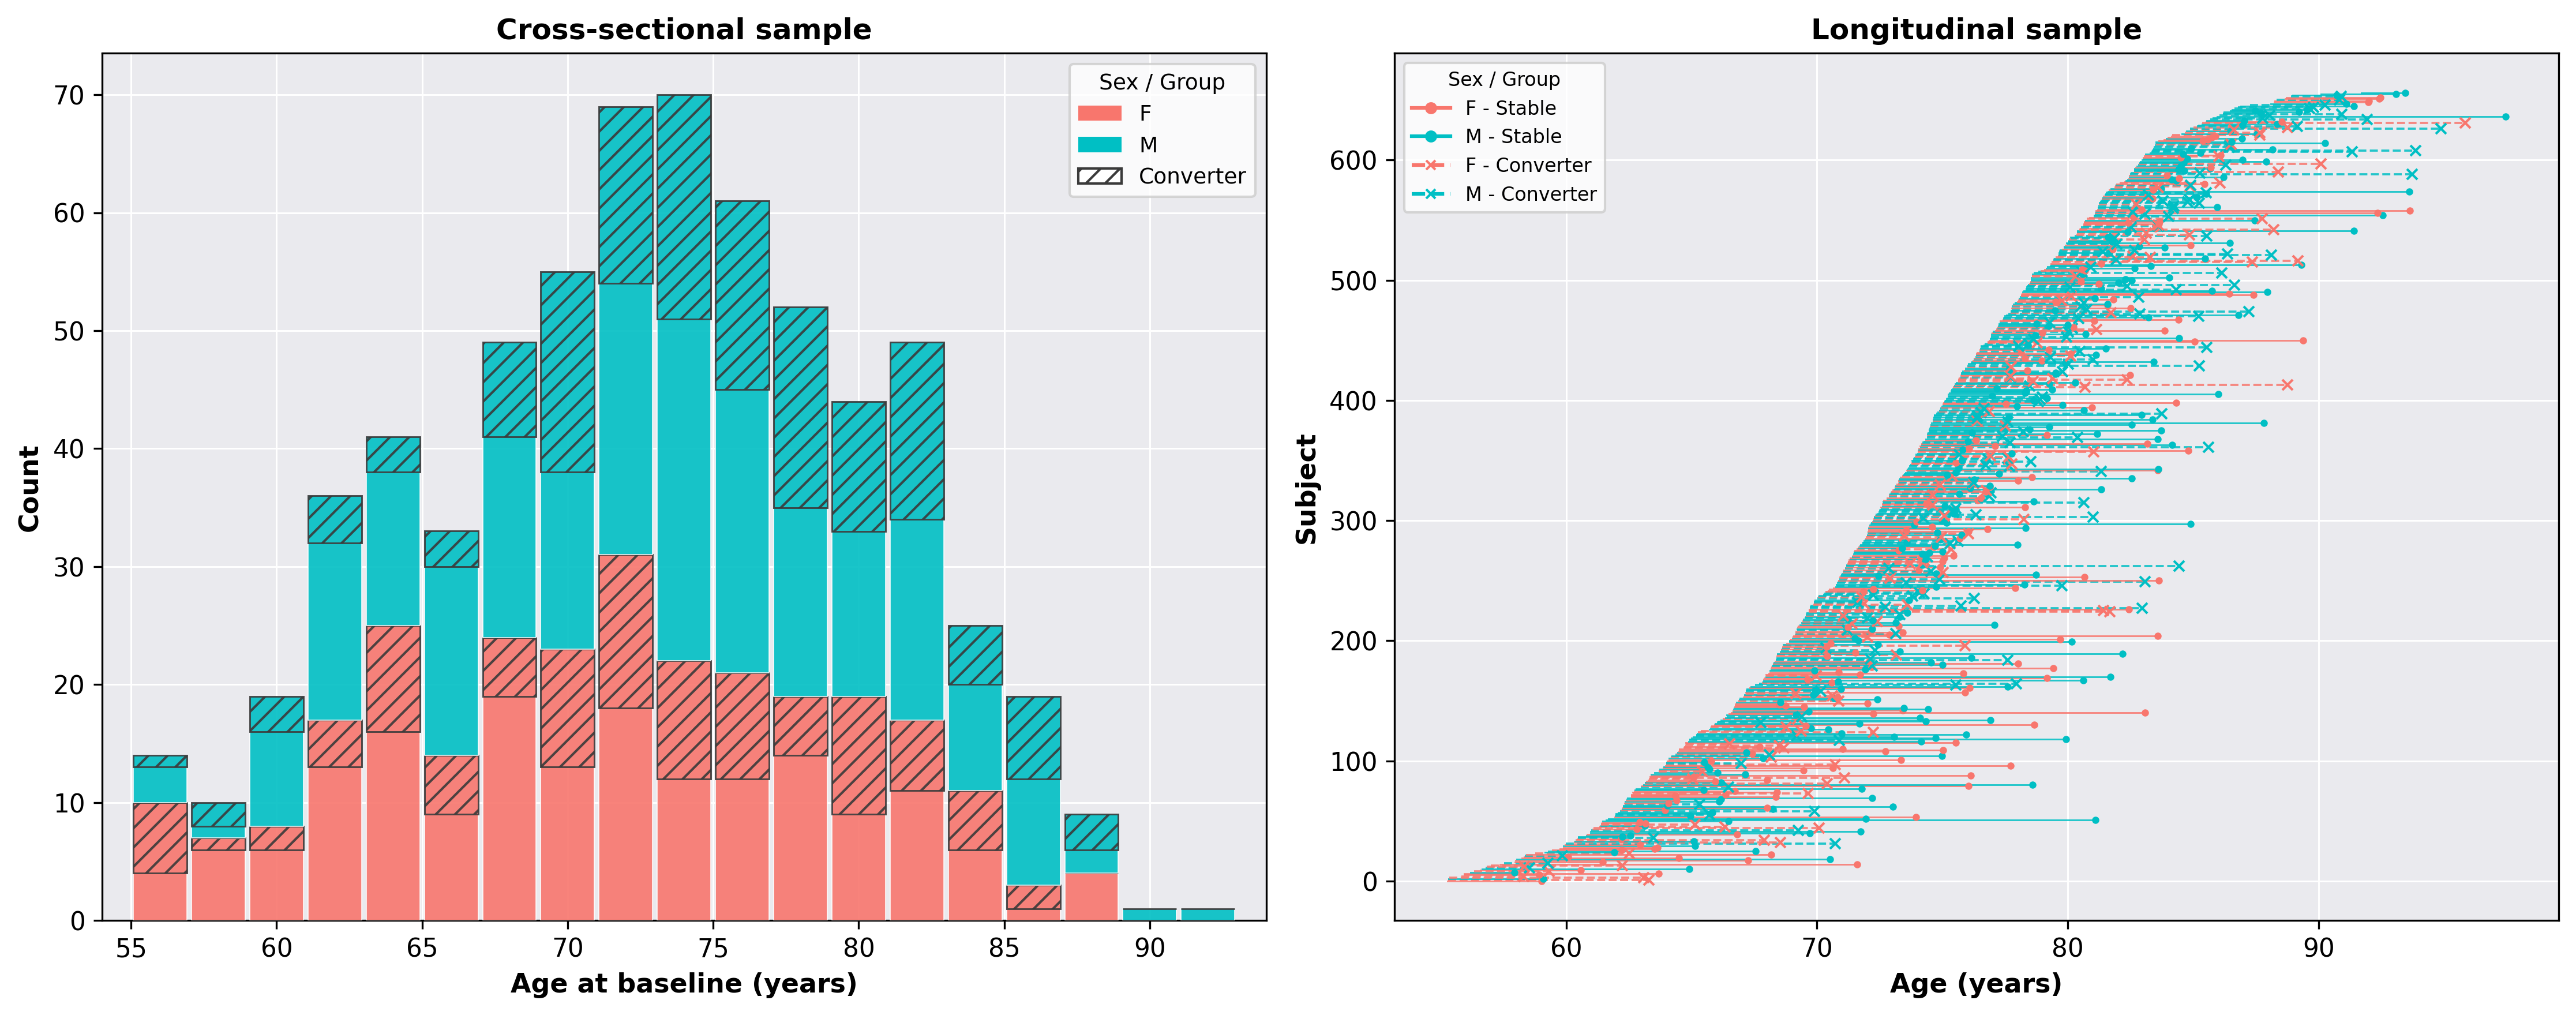
\includegraphics[width=0.95\textwidth]{Trillium/sample_overview_trillium.png}
\caption{Demographic and longitudinal sampling structure of the full processed ADNI series, before the landmark exclusions of Section~\ref{sec:landmark} are applied. \textbf{Left:} Cross-sectional age distribution at baseline, stacked by sex (salmon = Female, teal = Male); hatched portions indicate converters (MCI$\to$AD). \textbf{Right:} Longitudinal follow-up span for each subject, sorted by baseline age to reveal the S-shaped enrollment structure. Each horizontal line spans from baseline age to last available scan. Color indicates sex; line style and end marker distinguish stable subjects (solid line, circle) from converters (dashed line, $\times$). Converters are distributed across the full age range but cluster at shorter follow-up intervals, consistent with earlier event occurrence.}
\label{fig:sample-overview}
\end{figure*}
}

\subsubsection{External Validation Cohort}

Independent validation used the Open Access Series of Imaging Studies (OASIS-3). The identical preprocessing, BSC, and morphometry pipeline was applied, with conversion status derived from Clinical Dementia Rating trajectories rather than ADNI diagnosis codes. After processing, \textbf{79 subjects} with \textbf{18 conversion events} had complete features. That is a small cohort, and the confidence intervals below are correspondingly wide.

\subsection{MRI Acquisition and Preprocessing}

ADNI participants underwent T1-weighted structural MRI on 1.5T or 3T scanners using standardized acquisition protocols~\cite{jack2008adni_mri}. Scans were acquired with 3D magnetization-prepared rapid gradient-echo (MPRAGE) sequences across sites, with typical parameters of TR = 2300 ms, TE = 2.98 ms, TI = 900 ms, flip angle = 9$^\circ$, and isotropic voxel size of 1$\times$1$\times$1 mm$^3$. These settings are widely used because they provide good gray-white matter contrast without excessive scan time.

The BSC pipeline included several preprocessing steps. First, \textbf{N4 bias correction}~\cite{tustison2010n4} was applied to reduce low-frequency intensity non-uniformity caused by magnetic field inhomogeneity. Without that correction, gradual brightness shifts across the image could be mistaken for biologically meaningful boundary changes. N4ITK was run using default convergence settings (threshold: 0.001) and multi-resolution optimization across four levels ([50,50,50,50] iterations).

Next, \textbf{skull stripping} removed non-brain tissues such as skull, scalp, and orbital structures, which otherwise can interfere with segmentation and boundary detection. An Otsu-thresholding approach with morphological cleanup, including largest connected component selection and hole filling, was used. More advanced deep learning skull-stripping methods exist, such as SynthStrip and HD-BET~\cite{hoopes2022synthstrip}, and in some contexts they may perform better. However, the present pipeline prioritized speed, reproducibility, and minimal dependence on external training data.

All images were then \textbf{resampled to 1 mm$^3$ isotropic resolution} using linear interpolation. This step standardized spatial resolution across acquisitions and made voxel-wise comparisons more consistent. Linear interpolation was selected because it avoids some of the ringing artifacts that can appear with higher-order interpolation methods, which is relevant when gradients are later computed.

\textbf{Tissue segmentation} was performed using Atropos $k$-means clustering~\cite{avants2011atropos} with three classes corresponding to gray matter (GM), white matter (WM), and cerebrospinal fluid (CSF). The choice of $k$-means over alternatives such as Gaussian mixture models or deep learning segmentation was mainly pragmatic. It is fast, deterministic enough for reproducible workflows, and generally adequate for T1-weighted tissue separation in large cohorts. Each voxel was assigned class probabilities summing to 1.0, with $P_{GM}(\mathbf{x})$ denoting the gray matter probability at voxel $\mathbf{x}$.

\textbf{Boundary identification} was based on voxels satisfying $0.4 \leq P_{GM} \leq 0.6$, thereby defining a transition band centered around the gray-white matter interface~\cite{olafson2021bsc}. A single exact contour might seem cleaner in theory, but in practice it can be unstable and highly sensitive to noise.

\textbf{Gradient computation} used 3D Gaussian derivative filters with $\sigma = 1.0$ mm to estimate spatial derivatives of both MRI intensity $I(\mathbf{x})$ and gray matter probability $P_{GM}(\mathbf{x})$. The smoothing helps suppress high-frequency noise while preserving edge-related information. This produces gradient vectors $\nabla I$ and $\nabla P_{GM}$ at each voxel. Finally, \textbf{directional projection} extracted the component of the intensity gradient aligned with the boundary normal by taking the dot product with the normalized gray matter probability gradient. In effect, this isolates intensity change across the boundary rather than along it.

\subsection{Longitudinal Slope Computation}

For each scan, 33 BSC summary features were extracted across several categories (Table~\ref{tab:bsc-features}). These included boundary count, directional and magnitude-based summary statistics, percentile measures, and spatial bin summaries. To model longitudinal change, each feature was regressed against time within subject.

\begin{table}[htbp]
\centering
\caption{BSC feature categories extracted per scan}
\label{tab:bsc-features}
\begin{tabular}{lc}
\hline
\textbf{Feature Category} & \textbf{Count} \\
\hline
Boundary count (Nboundary) & 1 \\
Directional statistics (mean, std, median) & 3 \\
Directional percentiles (p10, p25, p50, p75, p90) & 5 \\
Magnitude statistics (mean, std, median) & 3 \\
Magnitude percentiles (p10, p25, p50, p75, p90) & 5 \\
Directional spatial bins (8 bins) & 8 \\
Magnitude spatial bins (8 bins) & 8 \\
\hline
\textbf{Total per scan} & \textbf{33} \\
\hline
\end{tabular}
\end{table}

For subject $s$ with scans acquired at times $t_1, t_2, t_3, t_4, \ldots$, longitudinal slopes for each feature $f$ were estimated using linear regression:

\begin{equation}
    f_s(t) = \beta_0 + \beta_1 \cdot t + \epsilon
\end{equation}

where $\beta_1$ represents the annualized rate of change. Reconstructed acquisition dates, rather than nominal visit codes, were used as the time variable so that irregular spacing between scans was captured accurately. The regression is fit only over scans inside the landmark window, so a subject who converted at month 30 contributes a slope estimated from scans at months 0, 12, and 24 and nothing later.

For each of the 33 base features, four primary longitudinal descriptors were derived: baseline value ($f_{\text{baseline}}$), final value ($f_{\text{final}}$), annual slope ($\beta_1$), and goodness-of-fit ($R^2$). Together these yielded \textbf{132 derived features} (4 $\times$ 33) per subject. The 33 annual slope terms and the 33 baseline values were carried forward as the slope and baseline feature sets respectively.

These 33 summaries are global, computed over the whole cortical ribbon, and one might reasonably ask why the analysis does not simply use regional coefficients from a cortical parcellation. Two reasons. The BSC pipeline used here segments tissue probabilistically and never builds a cortical surface, so it has no parcellation to project onto without adding a registration step, and its own failure modes, to every scan in the series. And with 160 events, a regional model would move from 33 summaries to several hundred correlated coefficients, which is the wrong direction for a cohort this size~\cite{riley2019minimum}. The spatial bin summaries are a coarse compromise: they divide the boundary voxels into eight spatial octants, which retains some topography at a fraction of the parameter cost. A properly regional analysis is worth doing and is listed among the future directions, but it is a different study.

\subsection{Feature Selection and Preprocessing}

The raw slope features showed extreme heterogeneity in variance. In particular, Nboundary\_slope, which reflects the rate of change in boundary voxel count, varied on a scale far larger than most other features. Left untreated, that imbalance risked allowing a single feature family to dominate downstream model behavior.

To address this, a feature selection and preprocessing pipeline was designed with robustness in mind. Selection was carried out on the training data only, inside each cross-validation fold, to avoid information leakage. First, raw slope values were transformed using a signed logarithm, $\text{sign}(x) \cdot \log(1 + |x|)$, which compresses extreme values while preserving the direction of change. Next, outliers were clipped by winsorization~\cite{winsorization} at the 1st and 99th percentiles, with those limits fit on the training set and then applied to the test set. Variance ranking was then computed on these robustly transformed features.

Because Nboundary-derived measures still tended to overwhelm the ranking, a \textbf{0.10 penalty factor} was applied to boundary count features during the selection step. This penalty altered the ranking scores only, not the actual feature values used for modeling. The goal was not to remove boundary count information, which may be biologically meaningful, but to prevent the model from reducing the analysis to a near-univariate problem.

After ranking, the top 20 features were retained. These selected features were passed through the same signed-log and winsorization steps, followed by MinMax scaling to the range [0, 1]. All transformation parameters were estimated on the training set alone and then transferred to the test set. After preprocessing, feature variances in the training data ranged from 0.019 to 0.157, a ratio of 8.2:1, compared with an original raw variance ratio near $6\times10^{9}$:1. That reduction substantially improved numerical balance across inputs while keeping directional interpretation intact.

\subsection{T1 Morphometry: The Established-Measure Comparator}

BSC describes one property of one interface. It says nothing about how much tissue is left, or whether the brain as a whole is shrinking, and reviewers of the earlier version rightly asked whether BSC slopes beat the conventional longitudinal MRI measures that any group would compute first. To answer that, T1 morphometry was extracted from exactly the same scans, inside exactly the same landmark window, and treated as a competing block rather than as an accessory to BSC.

Eight scan-level quantities were measured at every timepoint: total brain volume, brain parenchymal fraction (BPF, computed as [GM + WM] / TIV), total gray matter volume, total white matter volume, cerebrospinal fluid volume, mean brain signal intensity, signal-to-noise ratio, and brain-to-background intensity ratio. Brain volume loss and BPF decline are the standard structural markers of global neurodegeneration, and CSF volume carries ventricular expansion; the intensity and noise measures are quality descriptors included so that their contribution can be separated from the anatomical ones rather than silently absorbed.

Each of those eight was summarized twice. The \textbf{cross-sectional block} takes the value at the first scan in the window, plus TIV, brain mask volume, intensity standard deviation, and field strength at that scan, for 12 features. The \textbf{longitudinal block} takes six trajectory summaries per quantity over the window (value at the last in-window scan, absolute change, percent change, annual slope, mean, and standard deviation across scans), for 48 features. Every one of these is recomputed inside the landmark window for this revision. In the submitted analysis the trajectory summaries were computed over all scans up to and including the conversion visit, which means the T1 block was contaminated in the same way as the BSC block.

Two exclusions are worth recording. The upstream feature table carries the number of scans used per subject, which correlates with observed survival time at $r = 0.82$ because follow-up length determines both, so it is never used. And field strength as recorded in the DICOM headers contains a units error for a subset of scans, where 1.5T appears as 15000; these were rescaled before use, and 4.3\% of subjects changed field strength during their window.

\subsection{Clinical Covariates}

The clinical reference model uses four variables measured at or before the landmark: age at the landmark date, sex, years of education from ADNI demographics, and MMSE from the clinical visit closest to the landmark within a one-year window. MMSE was missing for 21 of 557 subjects and was imputed to the training-fold median.

These are deliberately unambitious. They are the variables a memory clinic already has, they cost nothing to collect, and both systematic reviews of this literature find that cognitive testing plus demographics is hard to beat~\cite{ansart2021predicting,grueso2021machine}. Any imaging marker that cannot improve on them has not yet earned a place in a prediction model, whatever its C-index looks like in isolation. Reporting an imaging model without this comparator, as the submitted version did, makes the marker look far more useful than it is.

\subsection{Survival Data Preparation}

Survival outcomes were defined using clinical diagnosis trajectories from DXSUM, as described in Section~\ref{sec:landmark}. For each subject, the first clinical visit at which the diagnosis reached dementia was treated as the conversion event, and time was measured from the landmark date to that visit. Subjects who never converted were right-censored at their last clinical visit, which is generally later than their last MRI.

This setup assumes that follow-up ended administratively rather than for reasons tied to future risk, conditional on observed covariates. That assumption cannot be verified directly, and any survival analysis quietly depends on it.

The final survival distribution included \textbf{160 conversion events}, with median time to conversion of 1.77 years from the landmark, and \textbf{397 censored subjects} with median follow-up of 2.63 years. The longer follow-up among censored subjects is expected, since individuals who do not convert continue contributing observation time.

\subsection{Statistical Analysis}

\subsubsection{Survival Modeling}

Six model families were fit on identical folds, and no single one is treated as primary. The point of the comparison is that a conclusion which holds only under one model class is a statement about that class rather than about the biomarker.

\textbf{Penalized Cox regression} is included at the reviewers' suggestion and is the natural default for this problem. With up to 84 candidate predictors and 160 events, an unpenalized Cox fit is unstable, so an elastic net penalty was used~\cite{simon2011regularization,cox1972} with $\ell_1$ ratio 0.5 over a 50-point regularization path, taking the midpoint of the path as the operating penalty. The proportional hazards assumption was checked with scaled Schoenfeld residuals on the fitted covariate-plus-BSC model.

\textbf{Parametric AFT models} under Weibull, log-normal, and log-logistic error distributions are the interpretable comparators, all three reported for every feature set rather than only the best of them.

\textbf{Random Survival Forest (RSF)} and \textbf{XGBoost with an AFT objective}~\cite{chen2016xgboost,barnwal2022survivalxgb} cover the nonlinear case. The two overfit differently, so agreement between them is more informative than either alone.

RSF extends the Random Forest framework to right-censored time-to-event data. Unlike parametric survival models, which impose a specific distribution on survival times, or Cox models~\cite{cox1972}, which rely on proportional hazards assumptions, RSF is \textit{non-parametric}. It does not require a prespecified hazard shape and is well suited to settings where the underlying relationships may be nonlinear or heterogeneous. For AD progression, that flexibility is attractive. Patients do not all decline in the same way, and it would be optimistic to assume a single hazard structure fits everyone cleanly.

Following Ishwaran et al.~\cite{ishwaran2008rsf}, the RSF algorithm builds an ensemble of survival trees using bootstrap samples of the training data. Each tree is grown by recursively splitting nodes based on a random subset of candidate features, with splits chosen to maximize survival differences between daughter nodes, typically using log-rank criteria. This randomness in both subjects and features helps reduce overfitting relative to a single decision tree.

For tree $b$ and subject $\mathbf{X}_i$, the cumulative hazard function was estimated within the terminal node containing that subject using the Nelson-Aalen estimator:

\begin{equation}
    \hat{H}_b(t | \mathbf{X}_i) = \sum_{t_j \leq t} \frac{d_j}{n_j}
\end{equation}

where $d_j$ is the number of events at time $t_j$ in the terminal node and $n_j$ is the number at risk. The ensemble cumulative hazard was then obtained by averaging across trees:

\begin{equation}
    \hat{H}(t | \mathbf{X}_i) = \frac{1}{B} \sum_{b=1}^{B} \hat{H}_b(t | \mathbf{X}_i)
\end{equation}

from which the survival function follows as $\hat{S}(t | \mathbf{X}_i) = \exp(-\hat{H}(t | \mathbf{X}_i))$.


In this implementation, RSF used 1,000 trees, minimum samples per split of 10, minimum samples per leaf of 15, and max features equal to $\sqrt{57} \approx 7.55 \rightarrow 7$ at each split on the combined feature set. These values were chosen based on common practice and computational feasibility rather than hyperparameter tuning.

\textbf{XGBoost} builds its ensemble differently. Where RSF grows independent trees on bootstrap samples and averages them, gradient boosting adds trees in sequence, each one fit to the residual error of the ensemble so far. That makes it more expressive than bagging on the same data, and correspondingly easier to overfit, which is the tradeoff visible in the results below.

Censoring was handled through XGBoost's \texttt{survival:aft} objective~\cite{barnwal2022survivalxgb}, which represents each subject as an interval rather than a point. A converter observed at time $t_i$ contributes the degenerate interval $[t_i, t_i]$; a censored subject last seen at $t_i$ contributes $[t_i, \infty)$. The model minimizes the negative log-likelihood of those intervals under a location-scale error model,

\begin{equation}
    \mathcal{L} = -\sum_{i=1}^{n} \log \left[ F\!\left(\frac{\log u_i - \hat{y}_i}{\sigma}\right) - F\!\left(\frac{\log l_i - \hat{y}_i}{\sigma}\right) \right]
\end{equation}

where $[l_i, u_i]$ is the observed interval for subject $i$, $\hat{y}_i$ is the ensemble's prediction of $\log T$, $F$ is the cumulative distribution of the assumed error term, and $\sigma$ is a fixed scale. A normal error distribution with $\sigma = 1.2$ was used. Because $\hat{y}$ predicts log survival time, higher predictions mean lower risk, and the concordance index was computed on $-\hat{y}$.

The model used 500 boosting rounds at a learning rate of 0.05, with maximum tree depth 4, minimum child weight 10, row subsampling 0.8, column subsampling 0.8, $L1$ penalty 0.1, $L2$ penalty 1.0, and seed 42. These settings lean toward regularization, and were fixed in advance rather than tuned, so no hyperparameter search was run against the test set.

For baseline comparison, Weibull, LogNormal, and LogLogistic AFT models were trained with L2 regularization (penalizer = 0.1). AFT models assume:

\begin{equation}
    \log(T) = \beta_0 + \sum_{i=1}^{p} \beta_i X_i + \sigma \epsilon
\end{equation}

where $T$ is survival time, $\beta_i$ are feature coefficients, $\sigma$ is a scale term, and $\epsilon$ follows the specified distribution. These models are attractive because their coefficients are interpretable, but they impose stronger assumptions that may not fit the biological heterogeneity of AD progression particularly well.

\subsubsection{Direction of the Risk Score}
\label{sec:direction}

The submitted version reported several C-index values below 0.5, and a reviewer correctly identified that a value below chance usually means the risk score has been read backwards. Every model here therefore returns a single quantity, defined so that larger always means earlier conversion, before any metric is computed. For the AFT models and for XGBoost, which predict survival time or its logarithm, the risk score is the negated prediction. For Cox it is the linear predictor. For RSF it is the predicted cumulative hazard. This convention is fixed once in the code and applied identically to every configuration, so a value below 0.5 in the results that follow reflects a model that genuinely fails to rank subjects, not a sign error. In practice, no configuration in the corrected analysis falls meaningfully below chance, which suggests the earlier sub-0.5 values came from a combination of direction handling and unstable parametric fits on a smaller sample.

\subsubsection{Model Training and Evaluation}

All configurations were evaluated by \textbf{5-fold cross-validation stratified by event status}, with feature selection, imputation, winsorization limits, and scaling refit inside each fold so that no held-out information reached the training process. The single 70/30 split used previously has been dropped as an evaluation device. With 160 events, a 30\% test set contains roughly 48 of them, and the fold-to-fold spread reported below is wide enough that any single split is close to uninformative. Cross-validation is used for every comparison, and the held-out predictions used for the Kaplan-Meier panels are out-of-fold predictions pooled across the five folds rather than predictions from one arbitrary split.

Discrimination was measured with the \textbf{concordance index}~\cite{uno2011cstat}, where 0.5 is random ranking. Because differences between feature blocks are small relative to fold-to-fold variation, block comparisons are made \textbf{within folds}: the two feature sets are fit on the same training partition and scored on the same held-out subjects, and the paired difference is what gets reported, with a bootstrap 95\% interval over folds and a paired $t$ test. Reporting two independent means with overlapping error bars would hide the pairing and understate the precision of the comparison.

Two further tests support the C-index comparisons. A likelihood ratio test compares the penalized Cox model with covariates plus BSC slopes against covariates alone, on the full cohort, which asks whether the slope block improves fit at all rather than whether it improves ranking. And univariable differences between converters and non-converters were computed for every selected slope, with false discovery rate control across features~\cite{benjamini1995controlling}.

\subsubsection{Comparison Groups}

Nine feature sets were compared: clinical covariates alone; BSC slopes alone; T1 cross-sectional alone; T1 longitudinal alone; the two T1 blocks together; BSC plus both T1 blocks; covariates plus BSC; covariates plus T1; and everything together. The covariates-only model is the reference against which the imaging blocks are judged. The T1 blocks answer whether BSC beats the established longitudinal measures. The combined sets answer whether it adds anything on top of them.

\subsubsection{The Effect of the Follow-up Definition}
\label{sec:design-methods}

To quantify how much of the previously reported performance came from the design rather than from the data, the entire pipeline was run a second time under the submitted follow-up definition, in which features come from every available scan and the clock starts at the MCI baseline. The two runs were then restricted to the same 557 subjects, with the same 160 events, so that cohort composition, features, model settings, folds, and seed are identical and the only difference is where follow-up starts.

\subsubsection{External Validation}

The XGBoost model fitted on ADNI was applied to OASIS-3 \textbf{without retraining}. Model weights, feature list, and preprocessing transform were held fixed: the winsorization limits and MinMax scaler fitted on ADNI training data were applied unchanged to the OASIS features, so they landed in the same feature space the model was trained on. A 95\% confidence interval on the external C-index was obtained by bootstrap resampling of subjects with 4,000 replicates.

One limitation of this transfer test should be stated up front. Per-scan BSC and morphometry features for OASIS-3 were computed on the cluster and are available here only as subject-level summaries, so the OASIS cohort could not be rebuilt under the landmark design. The external result therefore inherits the baseline follow-up definition and is reported as a transfer check on the earlier model rather than as external validation of the landmark analysis. Given that the landmark analysis finds no internal signal to transfer, rerunning it externally would test very little; the correct next step is a landmark-consistent external cohort, which is listed under future directions.

\subsection{Sample Size and Precision}

The post-hoc power calculation reported in the submitted version has been removed. Computing power after the fact from the observed effect adds nothing to the confidence intervals already reported, and power for a hazard ratio is in any case the wrong quantity for a study whose endpoint is out-of-sample discrimination. What follows instead is a statement of the precision this cohort supports.

With 557 subjects and 160 events, the 5-fold cross-validated C-index estimates carry a fold-to-fold standard deviation between 0.012 and 0.072 depending on configuration, which is the number reported alongside every point estimate. The paired block comparisons are more precise than those spreads suggest, since the pairing removes fold difficulty as a source of variance, and they resolve differences of roughly 0.013 in C-index.

Model complexity is the binding constraint on the larger feature sets. The full 84-feature matrix against 160 events gives 1.9 events per candidate predictor, well below what is needed for stable coefficient estimates~\cite{riley2019minimum}. The penalized Cox and ensemble models remain usable at that ratio, but individual feature importances should be read as suggestive. This is a further reason the analysis leans on block-level comparisons rather than on which particular slope ranked highest.

The external cohort remains the loosest estimate of all: 79 subjects with 18 events give a bootstrap interval roughly 0.25 wide.

\subsection{Software and Reproducibility}

All analyses were conducted in Python 3.11 using open-source tools. Preprocessing was performed with Advanced Normalization Tools (ANTs)~\cite{avants2011ants}, while survival modeling used scikit-survival~\cite{polsterl2020sksurv} for the Random Survival Forest and the elastic net Cox fit, XGBoost~\cite{chen2016xgboost} for the gradient-boosted AFT model, and lifelines~\cite{davidson-pilon2019lifelines} for parametric AFT models, the Cox hazard ratio table, the proportional hazards check, and Kaplan-Meier estimation. Clinical covariates were read from the ADNIMERGE2 tables with pyreadr. The landmark cohort construction, the model grid, the supplementary tests, and the figures are in \texttt{build\_landmark\_cohort.py}, \texttt{run\_revision\_models.py}, \texttt{revision\_supplementary.py}, and \texttt{make\_revision\_figures.py} respectively, each runnable from the cohort CSV. Segmentation and BSC computation for the full cohort were run on the Trillium high-performance computing cluster. Code for the full pipeline is available at \texttt{github.com/ishaan-cherukuri/research} and is intended to be made public upon acceptance.

\section{Results}

\subsection{Survival Model Performance}

\begin{table*}[!htbp]
\centering
\caption{Cross-validated discrimination by feature block and model family under the landmark design}
\label{tab:model-performance}
\begin{tabular}{llcccc}
\hline
\textbf{Feature set} & \textbf{Model} & \textbf{$p$} & \textbf{Train} & \textbf{Test} & \textbf{Gap} \\
\hline
Clinical covariates & Penalized Cox & 4 & 0.741 & 0.741$\pm$0.031 & 0.000 \\
Clinical covariates & Weibull AFT & 4 & 0.745 & 0.745$\pm$0.025 & 0.000 \\
Clinical covariates & Log-normal AFT & 4 & 0.746 & \textbf{0.747$\pm$0.024} & $-$0.001 \\
Clinical covariates & Log-logistic AFT & 4 & 0.745 & 0.745$\pm$0.024 & 0.000 \\
Clinical covariates & RSF & 4 & 0.789 & 0.725$\pm$0.033 & 0.064 \\
Clinical covariates & XGBoost AFT & 4 & 0.888 & 0.677$\pm$0.051 & 0.211 \\
\hline
BSC slopes & Penalized Cox & 20 & 0.573 & 0.523$\pm$0.049 & 0.050 \\
BSC slopes & Weibull AFT & 20 & 0.584 & 0.546$\pm$0.046 & 0.038 \\
BSC slopes & Log-normal AFT & 20 & 0.584 & 0.552$\pm$0.048 & 0.032 \\
BSC slopes & Log-logistic AFT & 20 & 0.589 & 0.556$\pm$0.045 & 0.032 \\
BSC slopes & RSF & 20 & 0.844 & 0.501$\pm$0.048 & 0.342 \\
BSC slopes & XGBoost AFT & 20 & 0.965 & 0.507$\pm$0.072 & 0.458 \\
\hline
T1 cross-sectional & Penalized Cox & 12 & 0.599 & 0.574$\pm$0.049 & 0.026 \\
T1 longitudinal & RSF & 48 & 0.866 & 0.579$\pm$0.035 & 0.287 \\
T1 morphometry (both) & RSF & 60 & 0.861 & 0.587$\pm$0.038 & 0.273 \\
BSC + T1 morphometry & RSF & 80 & 0.868 & 0.577$\pm$0.044 & 0.291 \\
\hline
Covariates + BSC & Penalized Cox & 24 & 0.742 & 0.741$\pm$0.032 & 0.002 \\
Covariates + BSC & Weibull AFT & 24 & 0.757 & 0.745$\pm$0.012 & 0.012 \\
Covariates + T1 & Penalized Cox & 64 & 0.748 & 0.736$\pm$0.031 & 0.012 \\
Covariates + BSC + T1 & Penalized Cox & 84 & 0.749 & 0.737$\pm$0.031 & 0.012 \\
Covariates + BSC + T1 & Weibull AFT & 84 & 0.784 & 0.722$\pm$0.037 & 0.062 \\
Covariates + BSC + T1 & RSF & 84 & 0.884 & 0.682$\pm$0.048 & 0.202 \\
Covariates + BSC + T1 & XGBoost AFT & 84 & 0.990 & 0.665$\pm$0.027 & 0.325 \\
\hline
\multicolumn{6}{p{0.92\textwidth}}{\footnotesize Means over 5 stratified cross-validation folds; $\pm$ is the fold standard deviation; $p$ is the number of features; Gap is train minus test. All 38 configurations are reported in the supplementary results file (\texttt{supplementary\_cv\_results.csv}); the rows here are the best model per block plus the full model family for the two blocks that matter. Risk direction is fixed as described in Section~\ref{sec:direction}, so values near 0.5 indicate genuine failure to rank rather than an inverted score.} \\
\end{tabular}
\end{table*}

Performance across the model ladder is given in Table~\ref{tab:model-performance} and summarized in Figure~\ref{fig:model-comparison}. The result is straightforward, and it is not the one this study set out to find.

\textbf{Clinical covariates set a high bar.} Age, sex, education, and MMSE at the landmark reached a test C-index of 0.747$\pm$0.024 under a log-normal AFT, with the penalized Cox and other parametric fits within 0.006 of that. These four variables have a train-test gap of essentially zero, which is what a well-specified low-dimensional model looks like.

\textbf{Imaging on its own performs close to chance.} The best BSC slope model reached 0.556$\pm$0.045 (log-logistic AFT), and the tree ensembles on the same features reached 0.501 and 0.507 while fitting their training data at 0.844 and 0.965. That pattern, near-perfect training performance with held-out performance at chance, is memorization of noise. T1 morphometry did slightly better at 0.587$\pm$0.038 but remains far below the covariates. Combining BSC with T1 did not help: 0.577$\pm$0.044.

\textbf{Adding imaging to the covariates changes nothing.} Covariates plus BSC reached 0.745$\pm$0.012 against 0.747 for covariates alone. Covariates plus both T1 blocks reached 0.736$\pm$0.031, and everything together reached 0.737$\pm$0.031. The fold-matched comparisons make this precise. Adding the BSC block to the covariates changed the test C-index by $-0.000$ (95\% CI $-0.013$ to $+0.013$, paired $p=0.98$) under a Weibull AFT and by $+0.000$ ($-0.003$ to $+0.003$, $p=0.97$) under penalized Cox. Adding it on top of covariates and T1 changed performance by $-0.007$ ($-0.019$ to $+0.002$) and $+0.001$ ($0.000$ to $+0.002$) respectively. Under RSF the increment was reliably negative ($-0.033$, $-0.050$ to $-0.015$), which is what happens when 20 uninformative features are handed to a model that will split on them anyway.

\begin{figure*}[!htbp]
\centering
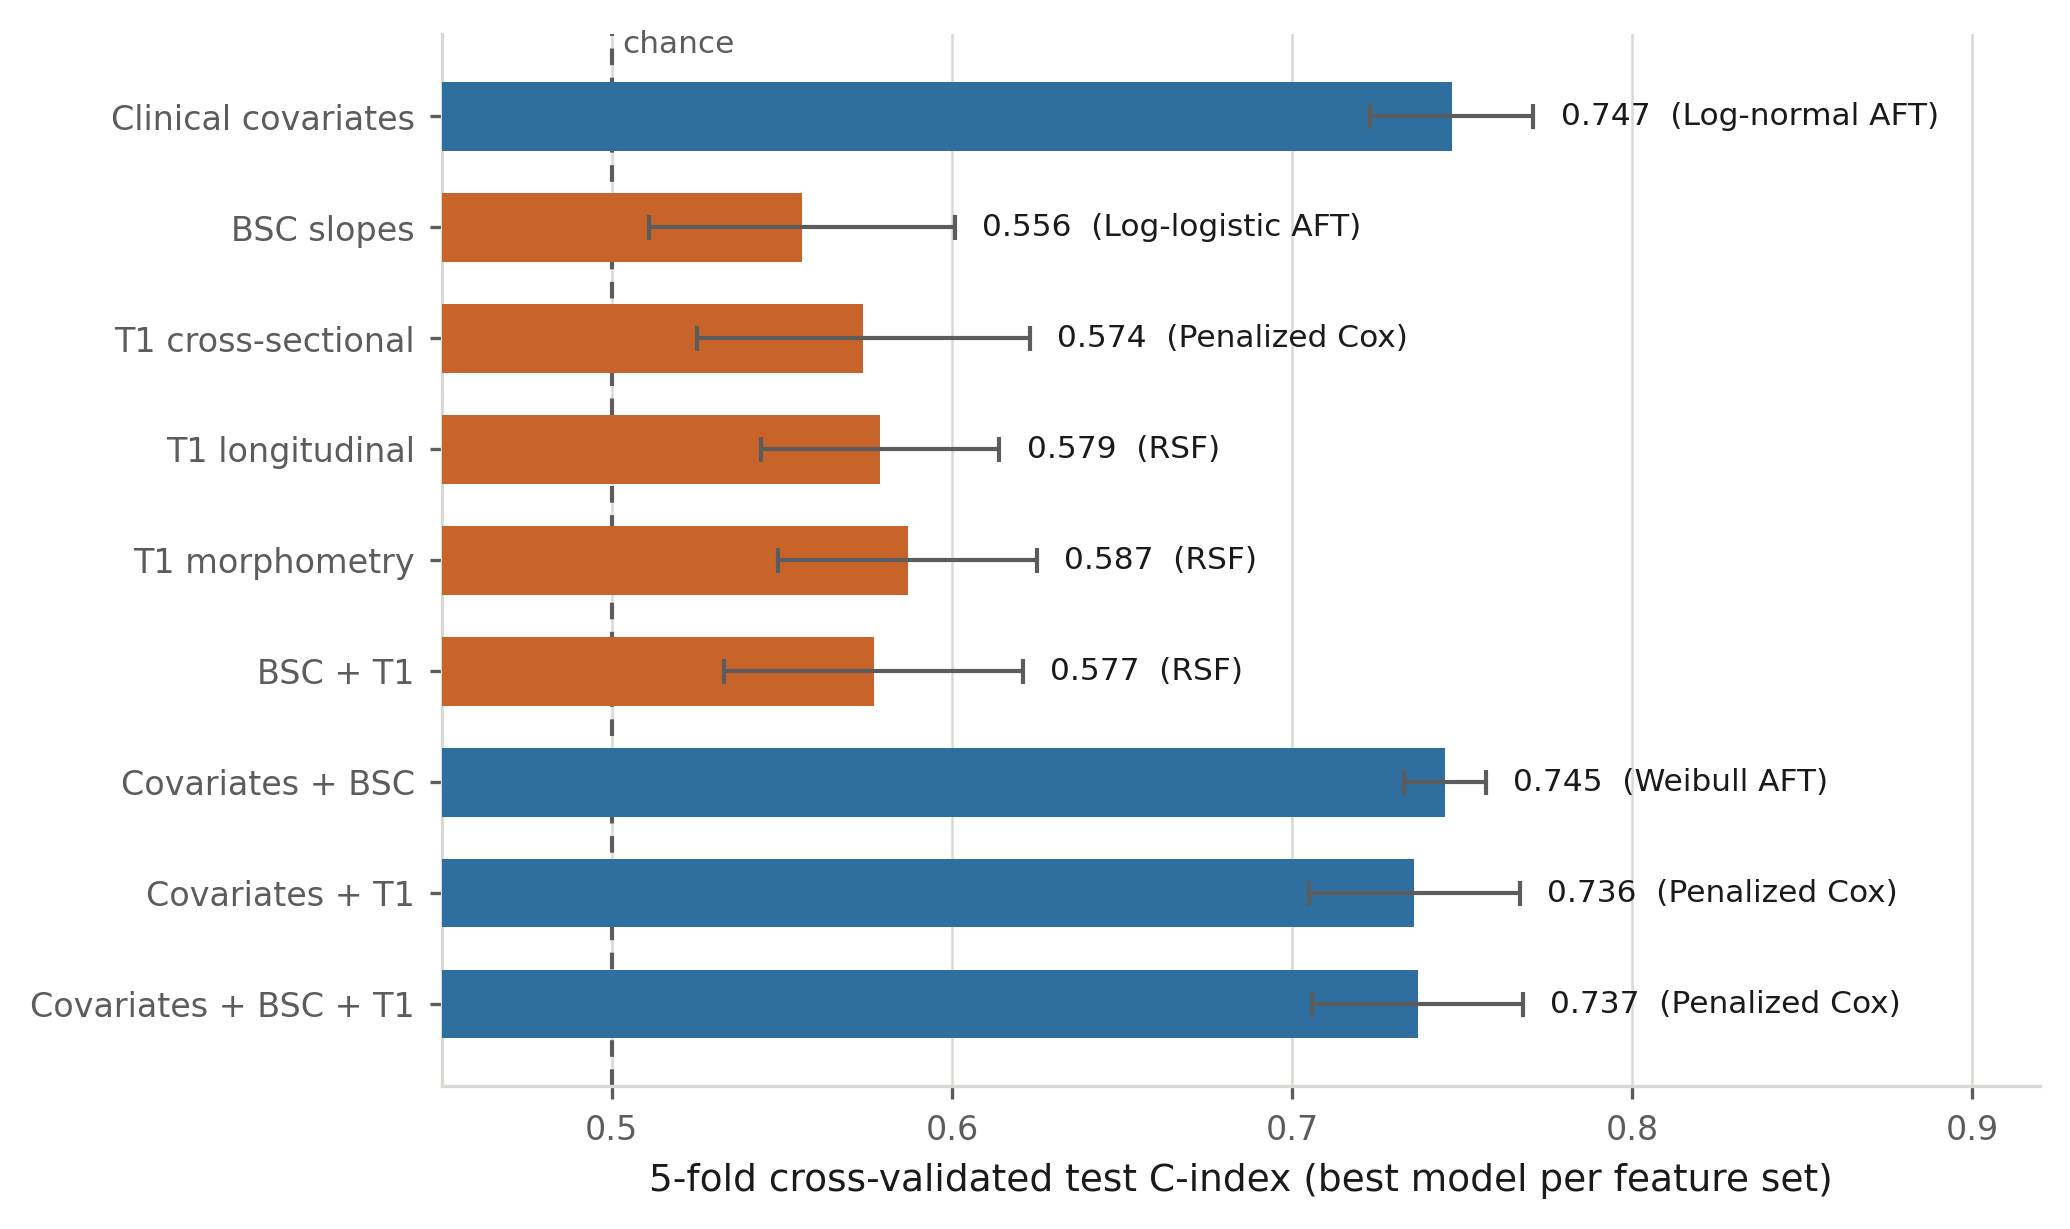
\includegraphics[width=0.95\textwidth]{revision/fig_landmark_models.png}
\caption{Cross-validated test C-index by feature set under the landmark design, showing the best-performing model family for each set with the fold standard deviation as error bars. Sets containing clinical covariates are shown in blue and imaging-only sets in orange. Every imaging-only configuration sits between 0.50 and 0.59, while every set containing age, sex, education, and MMSE sits near 0.74 regardless of what imaging is added to it. The dashed line marks chance.}
\label{fig:model-comparison}
\end{figure*}

The penalized Cox model fit on the full cohort tells the same story from the likelihood side. With covariates and the 20 selected slopes, concordance was 0.753 against 0.743 for covariates alone, and the slope block did not improve the partial likelihood ($\chi^2 = 5.08$ on 20 degrees of freedom, $p = 1.00$). Table~\ref{tab:cox-hr} gives the adjusted hazard ratios. MMSE and age carry the model; no BSC slope reaches significance, and the smallest slope $p$ value is 0.38. Scaled Schoenfeld residuals gave no evidence against proportional hazards (minimum $p = 0.28$ across terms).

Univariable comparisons agree. Converters had lower MMSE ($d=-0.71$, $p=1.0\times10^{-11}$) and were older ($d=0.37$, $p=8.1\times10^{-5}$). BSC slopes were more negative in converters, which is the expected direction, but the largest effect size was $d=-0.15$ and no slope survived false discovery correction across the 20 tested features (smallest $q = 0.66$).

\begin{table}[htbp]
\centering
\caption{Adjusted hazard ratios from the penalized Cox model, covariates plus the 20 selected BSC slopes}
\label{tab:cox-hr}
\begin{tabular}{lccc}
\hline
\textbf{Term} & \textbf{HR} & \textbf{95\% CI} & \textbf{$p$} \\
\hline
MMSE at landmark & 0.62 & 0.56--0.69 & $1.2\times10^{-18}$ \\
Age at landmark & 1.27 & 1.12--1.46 & $3.6\times10^{-4}$ \\
Nboundary slope & 1.07 & 0.92--1.25 & 0.38 \\
bsc\_dir\_bin\_5 slope & 0.92 & 0.73--1.16 & 0.49 \\
bsc\_mag\_p90 slope & 1.09 & 0.85--1.39 & 0.49 \\
bsc\_dir\_bin\_3 slope & 1.08 & 0.85--1.36 & 0.54 \\
\hline
\multicolumn{4}{p{0.44\textwidth}}{\footnotesize All predictors standardized, so hazard ratios are per standard deviation. The four leading BSC slopes are shown; the remaining 16, plus sex and education, had larger $p$ values. Likelihood ratio test for the whole 20-slope block against covariates alone: $\chi^2 = 5.08$, 20 df, $p = 1.00$.} \\
\end{tabular}
\end{table}

Kaplan-Meier curves built from out-of-fold predictions (Figure~\ref{fig:km-curves}) show the same thing visually. Risk tertiles separate cleanly in both panels, with log-rank $p<0.0001$ comparing outer tertiles, and the two panels are almost indistinguishable. The separation is real and it comes from the clinical variables. Adding 80 imaging features to the model does not move the curves.

\begin{figure*}[!htbp]
\centering
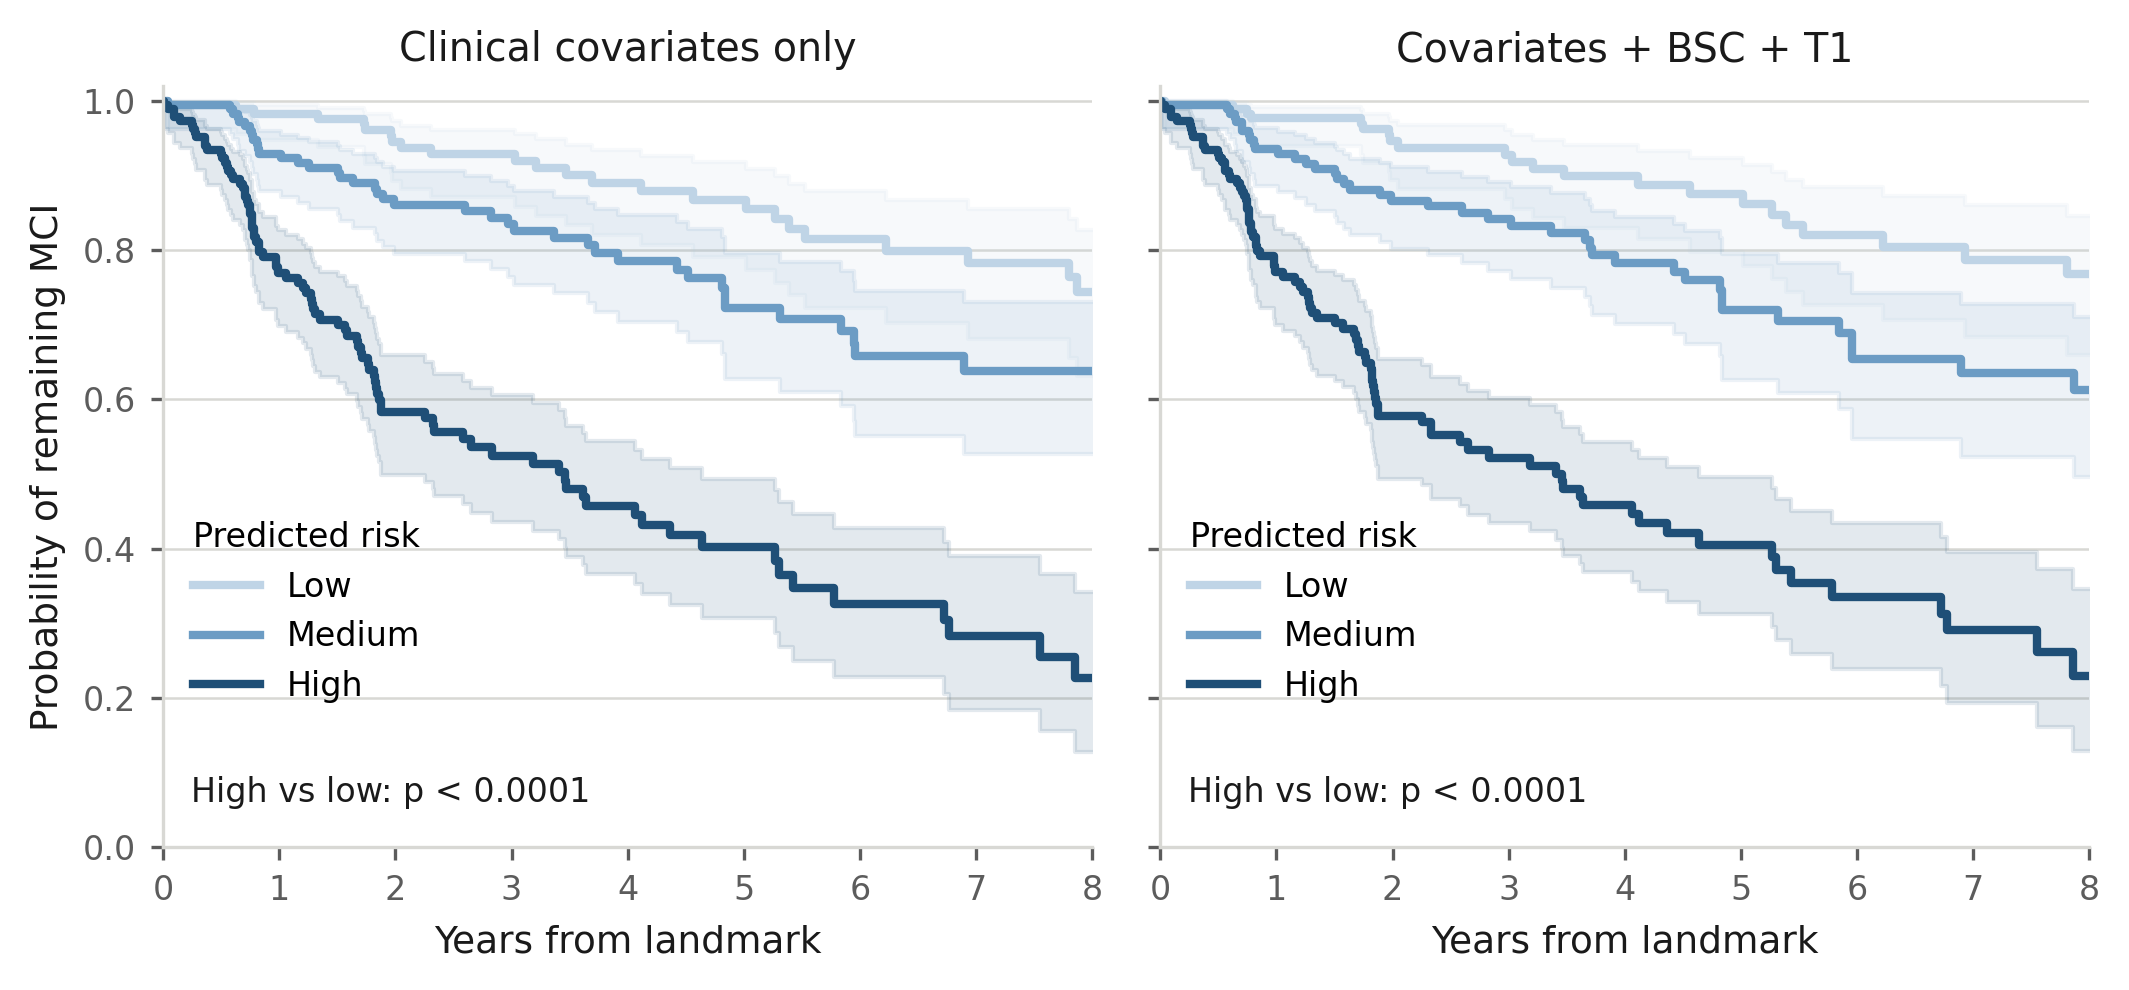
\includegraphics[width=0.95\textwidth]{revision/fig_landmark_km.png}
\caption{Kaplan-Meier curves by predicted-risk tertile under the landmark design, using out-of-fold predictions pooled across the five cross-validation folds so that every subject is scored by a model that did not see them. \textbf{Left:} penalized Cox on clinical covariates alone. \textbf{Right:} the same model with the BSC slopes and both T1 morphometry blocks added. Shaded bands are 95\% confidence intervals. Both panels separate strongly (log-rank on outer tertiles $p<0.0001$), and they separate to almost exactly the same degree, which is the visual form of the null increment reported in the text.}
\label{fig:km-curves}
\end{figure*}

\subsection{How Much Came From the Follow-up Definition}
\label{sec:design-effect}

The submitted analysis reported 0.645 for BSC slopes under RSF and 0.832 for the combined model. Those numbers came from the same scans and the same code as the ones above. What changed is where the clock starts.

Scoring the same 557 subjects under both definitions, and holding features, folds, hyperparameters, and seed fixed, the only difference is the follow-up definition (Section~\ref{sec:design-methods}). Under the submitted definition, BSC slopes reached 0.720 with RSF and 0.644 with a log-logistic AFT. Under the landmark definition, the same features in the same folds reached 0.501 and 0.556. T1 morphometry fell from 0.712 to 0.587, and the combined imaging model from 0.672 to 0.534. The clinical covariates went the other way, from 0.684 to 0.747, which is exactly what should happen: demographics and cognition do not depend on when the scans were taken, and the landmark cohort is slightly easier to rank because its follow-up window is better defined. Figure~\ref{fig:design-effect} shows the comparison.

\begin{figure*}[!htbp]
\centering
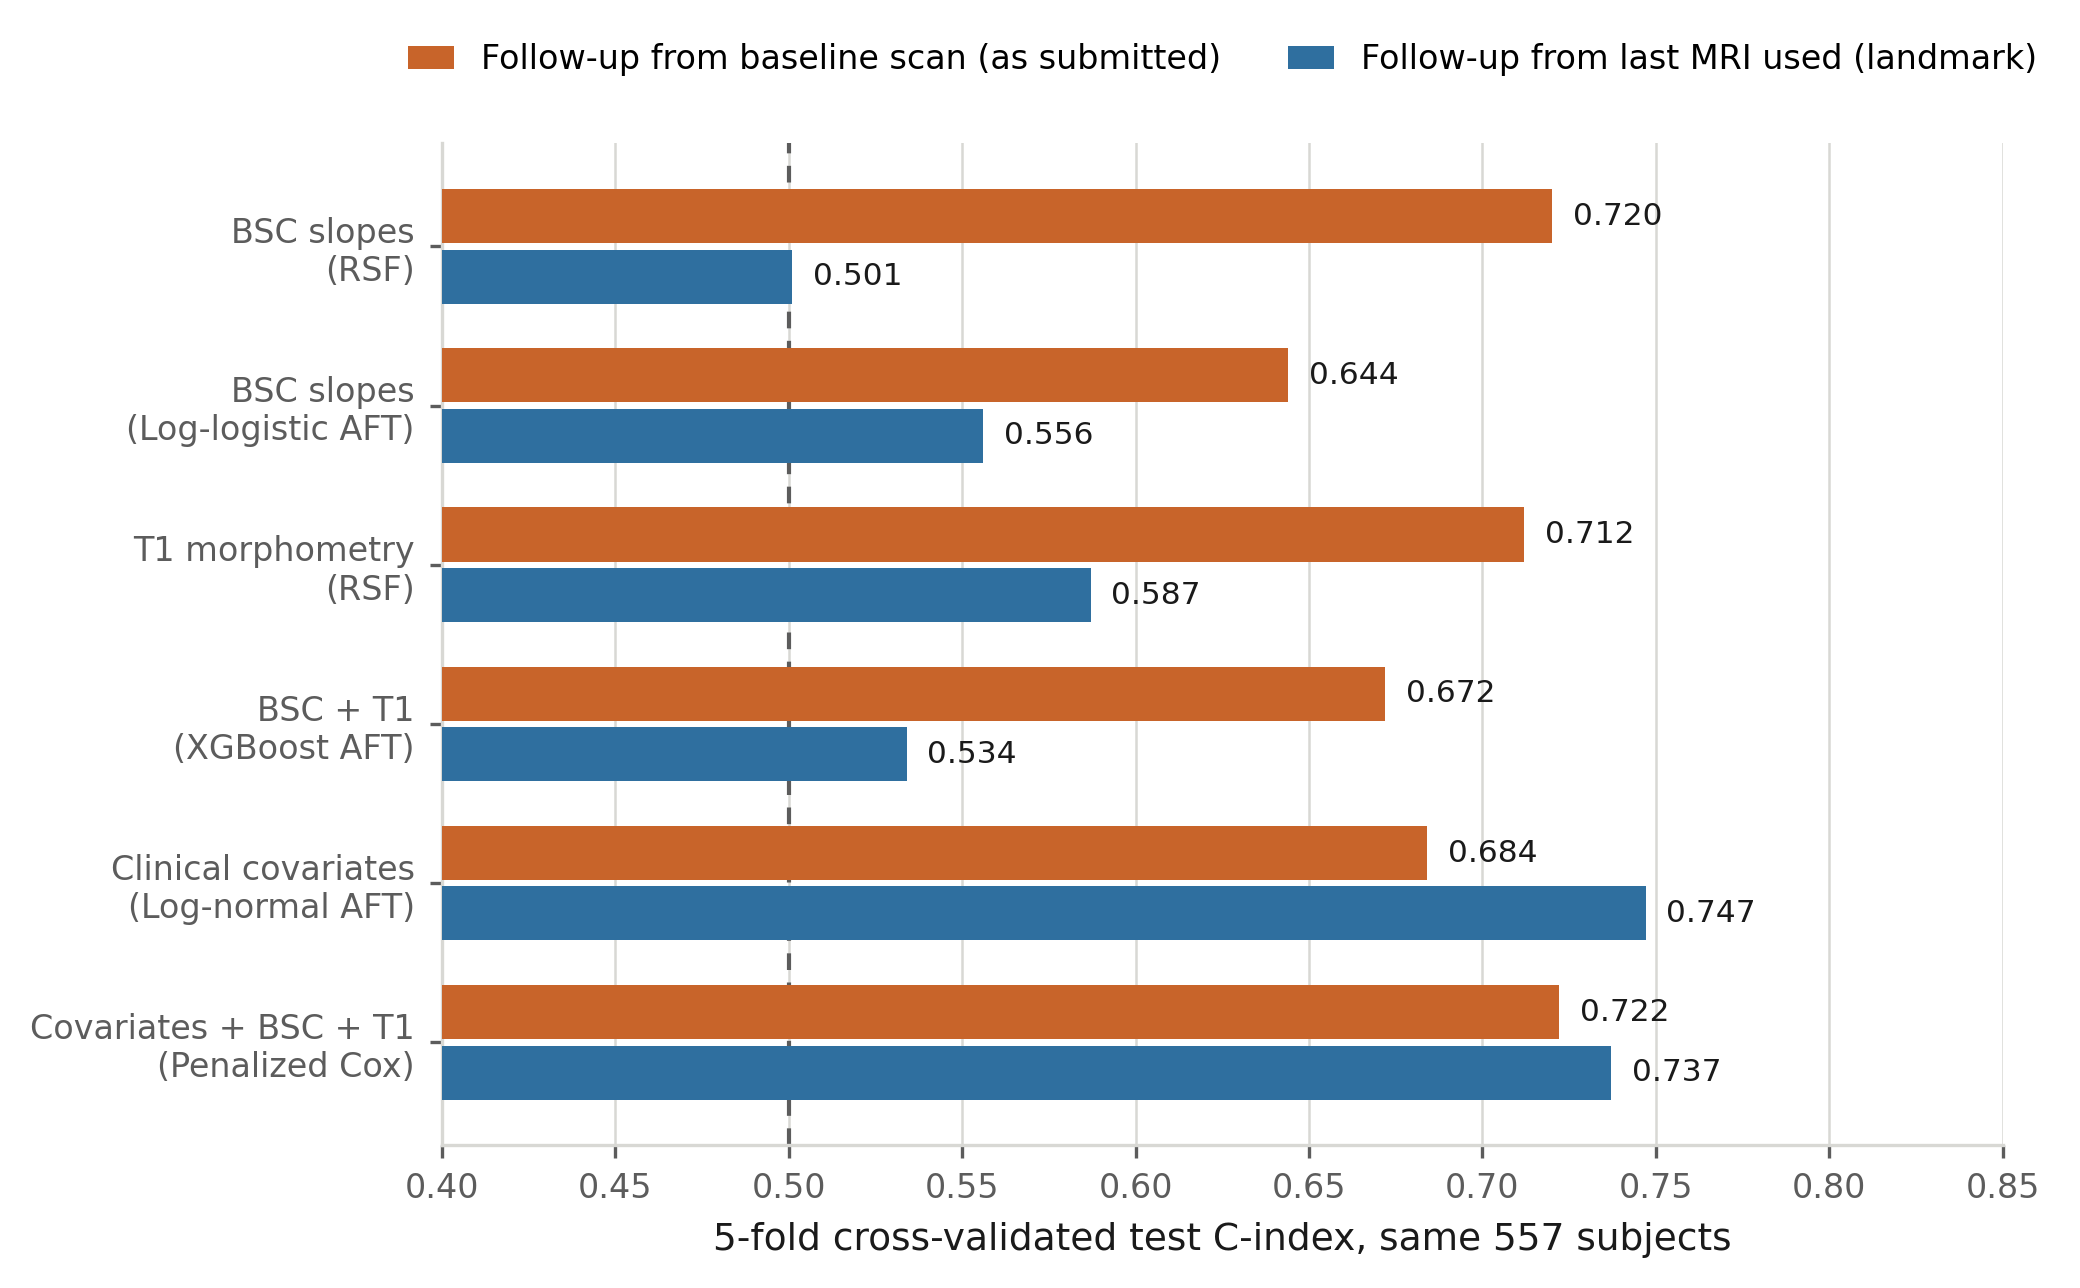
\includegraphics[width=0.95\textwidth]{revision/fig_design_effect.png}
\caption{Effect of the follow-up definition, holding everything else constant. The same 557 subjects, the same 160 events, and the same features, folds, hyperparameters, and random seed are scored under the submitted definition, where the clock starts at the MCI baseline scan and every scan contributes features (orange), and under the landmark definition, where features come only from scans acquired while the subject was still MCI and the clock starts at the last of them (blue). Imaging performance collapses toward chance under the corrected design while the clinical model is unaffected, which locates the earlier signal in the design rather than in the images.}
\label{fig:design-effect}
\end{figure*}

The interpretation is uncomfortable but not ambiguous. An imaging block whose apparent discrimination disappears when post-diagnosis scans are removed from the feature window was, to a large extent, reading the diagnosis rather than predicting it.

\subsection{Sensitivity to the Landmark Choice}
\label{sec:sensitivity}

The 24-month landmark is a design choice, so the analysis was repeated with the landmark placed at each subject's own last pre-conversion scan. That variant keeps 680 subjects and 272 events and uses more scans per subject, at the cost of much shorter and more variable follow-up (median 0.47 years), since a non-converter's last scan often falls close to their last clinic visit.

The conclusions do not change. Clinical covariates reached 0.761$\pm$0.036, BSC slopes 0.558$\pm$0.022 at best, T1 morphometry 0.569$\pm$0.038, and covariates plus BSC 0.752$\pm$0.035. Covariates plus all imaging and covariates plus T1 both reached 0.771$\pm$0.036, identical to three decimal places, which again places the BSC contribution at zero. Two different landmark definitions, two different cohorts, and the same answer.

\subsection{Dependence on Acquisition}
\label{sec:acquisition}

Section~\ref{sec:landmark} predicted that BSC would inherit the acquisition sensitivity of any gradient-based contrast measure. It does.

Mean BSC magnitude at the first in-window scan differed between field strengths, at 0.639 for 1.5T ($n=152$) against 0.590 for 3T ($n=397$), a difference of $d=0.30$ ($p=0.003$). It also correlated with baseline SNR ($r=0.22$, $p=1.8\times10^{-7}$). Both associations are modest in size, and neither is surprising for a measure built from an intensity gradient, but both are larger than any converter versus non-converter difference observed in the same cohort, where the largest effect size was $d=0.15$. When a scanner covariate moves a biomarker twice as much as the disease does, that biomarker needs harmonization before it is modeled, not after.

The annualized slope was affected as well. Mean BSC magnitude slope was $-0.021$ per year at 1.5T against $-0.005$ at 3T ($p=0.029$), so the apparent rate of boundary degradation depends partly on which scanner a subject happened to be imaged on. Field strength changed at least once during the landmark window for 4.3\% of subjects. In this cohort that is too small a subgroup to drive the main result, but in a study with more scanner turnover it would be a serious problem, and it argues for treating field strength as something to harmonize~\cite{fortin2018harmonization} rather than as a covariate to include and hope for the best.

\subsection{Feature Selection Ranking}

\begin{table}[htbp]
\centering
\caption{Top 10 BSC slope features selected by penalized robust variance}
\label{tab:top-features}
\begin{tabular}{lc}
\hline
\textbf{Feature} & \textbf{Variance} \\
\hline
Nboundary\_slope & 0.157 \\
bsc\_mag\_bin\_2\_mean\_slope & 0.030 \\
bsc\_mag\_bin\_0\_mean\_slope & 0.030 \\
bsc\_mag\_bin\_6\_mean\_slope & 0.030 \\
bsc\_mag\_p90\_slope & 0.029 \\
bsc\_mag\_bin\_4\_mean\_slope & 0.028 \\
bsc\_mag\_mean\_slope & 0.027 \\
bsc\_mag\_bin\_5\_mean\_slope & 0.027 \\
bsc\_mag\_median\_slope & 0.026 \\
bsc\_mag\_p50\_slope & 0.026 \\
\hline
\end{tabular}
\end{table}

\textit{Note: Variances shown after robust preprocessing pipeline (signed-log transform, winsorization, penalization, MinMax scaling to [0,1]). Nboundary features were penalized by 0.10 during selection ranking to prevent dominance while retaining complementary information. Final variance range: 0.019--0.157 (ratio 8.2:1), enabling balanced contribution across all features in the ensembles. This is the selection ranking, computed before any model was fit, and is distinct from the model-based importances in Table~\ref{tab:xgb-importance}.}

After preprocessing, the selected features showed a much more balanced variance structure. Nboundary\_slope retained the largest variance at 0.157, but it no longer overwhelmed the feature set. Several magnitude-based slopes, including spatial bin means and the higher percentiles, clustered in a similar range between 0.026 and 0.030. This is a variance ranking computed before any model is fit, so it says which features vary across subjects, not which ones carry prognostic information. Given the null result above, it should be read purely as documentation of what entered the models.

Model-based importance from the submitted analysis is retained below because it explains, in part, how the earlier result arose. Gain importance was computed from the fitted XGBoost booster by summing the loss reduction attributable to every split on each feature across all 500 trees (Table~\ref{tab:xgb-importance}). These values come from the model fit under the baseline follow-up definition, on the contaminated feature window, and are not importances for any model in Table~\ref{tab:model-performance}.

\begin{table}[htbp]
\centering
\caption{Top 10 features by XGBoost gain importance, as a percentage of total gain}
\label{tab:xgb-importance}
\begin{tabular}{llc}
\hline
\textbf{Feature} & \textbf{Block} & \textbf{Gain (\%)} \\
\hline
long\_brain\_bg\_ratio\_std & T1 & 15.8 \\
long\_brain\_vol\_std & T1 & 10.0 \\
long\_snr\_std & T1 & 9.3 \\
long\_snr\_slope\_yr & T1 & 6.7 \\
long\_brain\_vol\_slope\_yr & T1 & 4.9 \\
long\_brain\_bg\_ratio\_slope\_yr & T1 & 3.8 \\
long\_brain\_vol\_pctchg & T1 & 2.1 \\
bsc\_dir\_bin\_1\_mean\_slope & BSC & 2.0 \\
long\_brain\_intensity\_std & T1 & 2.0 \\
Nboundary\_slope & BSC & 2.0 \\
\hline
\multicolumn{2}{l}{\textbf{All 20 BSC slopes combined}} & \textbf{18.4} \\
\multicolumn{2}{l}{\textbf{All 37 T1 features combined}} & \textbf{81.6} \\
\hline
\end{tabular}
\end{table}

This distribution was uncomfortable for a study built around boundary sharpness even before the design was corrected. Only two BSC features appear in the top ten, and the whole slope block accounts for 18.4\% of total gain against 81.6\% for T1. The single largest contributor, the standard deviation of brain-to-background intensity ratio across a subject's scans, measures scan-to-scan signal variability rather than anatomy.

Read alongside Section~\ref{sec:design-effect}, the table becomes interpretable. The features doing the work were dispersion summaries computed over a scan series whose length and composition depend on when the subject was diagnosed. A subject who converted early has a short series with few scans; one who never converted has a long one. Any summary sensitive to series length or to the inclusion of a post-diagnosis scan therefore carries outcome information that has nothing to do with the brain. That is the mechanism behind the 0.83, and it is why removing post-conversion scans from the window costs the imaging blocks 0.10 to 0.20 C-index while leaving the clinical model untouched.

\subsection{External Validation}

Applied to 79 OASIS-3 subjects without retraining, the frozen model achieved a C-index of \textbf{0.623}, with a bootstrap 95\% confidence interval of \textbf{[0.501, 0.746]} (Figure~\ref{fig:external}). Internal cross-validated performance under the same baseline follow-up definition was 0.832$\pm$0.018, so transfer cost roughly 0.21. Both numbers belong to the uncorrected design, for the reason given in the methods, and the section is retained because the transfer failure turns out to be an early symptom of what Section~\ref{sec:design-effect} diagnoses directly. A model leaning on artifacts of a cohort's scan scheduling should not be expected to survive contact with a cohort scheduled differently.

\begin{figure*}[!htbp]
\centering
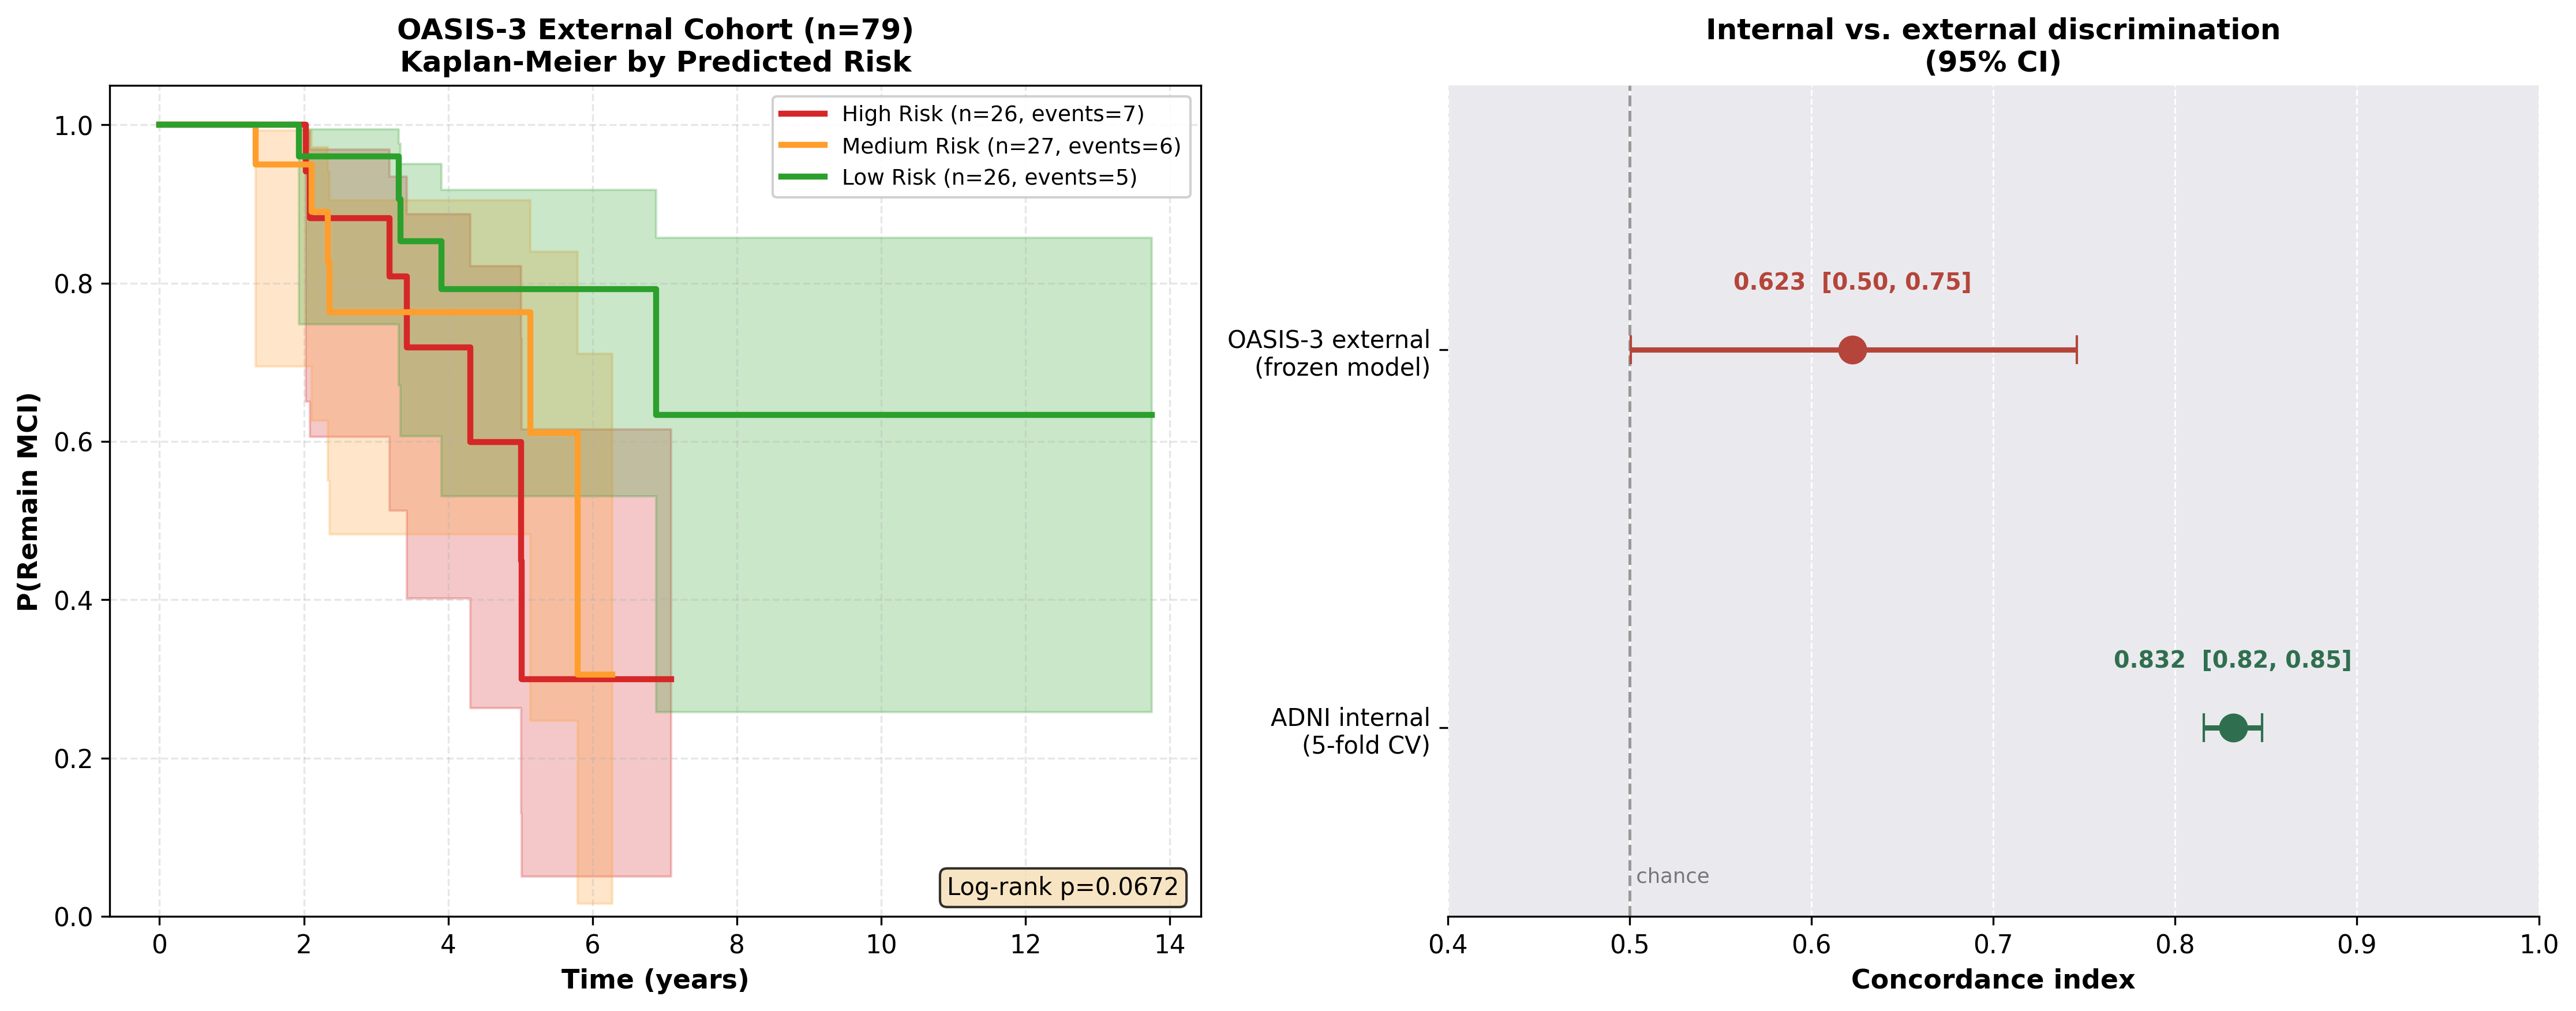
\includegraphics[width=0.95\textwidth]{Trillium/external_validation_oasis.png}
\caption{External validation on OASIS-3 (n=79, 18 events). \textbf{Left:} Kaplan-Meier curves by predicted-risk tertile. Event counts are 7, 6, and 5 across high-, medium-, and low-risk groups, and the curves overlap substantially; the log-rank comparison of outer tertiles is not significant ($\chi^2 = 3.35$, $p = 0.067$). \textbf{Right:} internal versus external discrimination with 95\% confidence intervals. Internal cross-validated performance is 0.832 [0.82, 0.85]; external performance is 0.623 [0.50, 0.75], with the lower bound at chance. Bootstrap resampling placed 2.5\% of replicates at or below 0.5.}
\label{fig:external}
\end{figure*}

The confidence interval is informative in two directions. Its lower bound sits at 0.501, so the external result is only marginally distinguishable from chance, with 2.5\% of bootstrap replicates falling at or below 0.5. Its upper bound reaches 0.746, so a genuinely useful level of discrimination is not ruled out either. With 18 events, this cohort cannot settle the question.

Risk stratification tells the same story more starkly. The predicted-risk tertiles contained 7, 6, and 5 events, an ordering in the right direction but far from the 41/18/17 split seen internally, and the log-rank test on outer tertiles was not significant ($p = 0.067$). Whatever the model learned on ADNI, most of it did not carry over.

For context, a test C-index of 0.62 sits at the low end of the range commonly reported for structural MRI-only prediction of MCI conversion, which the reviews place around 0.70 to 0.78 in AUC terms for imaging-only models~\cite{ansart2021predicting}. Under the landmark design the imaging blocks do not reach even that.

\section{Discussion}

\subsection{Principal Findings}

The headline finding is negative, and it is more useful than the positive one it replaces.

\textbf{Longitudinal BSC slopes add no prognostic information beyond routine clinical variables.} Age, sex, education, and MMSE at the landmark reach a cross-validated C-index of 0.747. Adding 20 BSC slopes moves that by $-0.000$ (95\% CI $-0.013$ to $+0.013$). Adding them on top of T1 morphometry as well moves it by $-0.007$. The Cox partial likelihood does not improve ($p=1.00$), no individual slope survives false discovery correction, and the result holds under two landmark definitions and six model families. This is not a case of an underpowered test failing to reach significance around a promising point estimate. The point estimate is zero.

\textbf{The earlier positive result came from the follow-up definition.} Holding subjects, features, folds, and seed fixed and changing only where the survival clock starts moves BSC slope performance from 0.720 to 0.501 and the combined imaging model from 0.672 to 0.534, while the clinical model is unaffected. The submitted analysis allowed scans acquired at or after the dementia diagnosis into the feature window and started follow-up before those scans were taken. Under that arrangement, features that encode how long a subject's scan series ran, or that include a post-diagnosis image, predict the outcome without carrying prognostic information. The gain table in the submitted version was already pointing at this: the top contributors were standard deviations across a subject's scan series, not anatomical measures.

\textbf{BSC is measurably sensitive to acquisition.} Field strength shifts baseline BSC magnitude by $d=0.30$ and shifts the annualized slope as well, and BSC tracks SNR at $r=0.22$. Both exceed any converter versus non-converter difference in the same cohort. A marker in that position is not ready to be modeled without harmonization.

Two things this study does not show are worth stating, because a null result invites over-reading. It does not show that the gray-white boundary is uninformative in AD. It shows that these global BSC summaries, over a two-year window, in this cohort, do not add to a clinical model. Regional measures, longer windows, surface-based contrast estimates, or harmonized acquisitions could all behave differently. It also does not show that imaging is useless for conversion prediction; the T1 morphometry block, measured over the same short window, was similarly flat, which points as much at the two-year window as at the markers.

The broader lesson is methodological and applies well beyond BSC. In a longitudinal biomarker study the analysis window and the follow-up window must not overlap, and when they do the resulting performance can look excellent. The reviews of this literature already flag design heterogeneity as a driver of reported performance~\cite{ansart2021predicting,grueso2021machine}. This study is a concrete instance: the same data supported a C-index of 0.83 and a null result depending only on where the clock started.

\subsection{Why External Performance May Have Dropped}

Several explanations fit the evidence, and they are not mutually exclusive.

The most likely one concerns what the top features are measuring. The three largest gain contributors are all standard deviations of image-derived quantities across a subject's scan series. These depend heavily on how consistently a subject was imaged, which is a property of a study's protocols and scanner fleet as much as of the subject's brain. ADNI and OASIS-3 differ in both. A model leaning on scan-to-scan variability would be expected to transfer poorly, and that is what happened.

Outcome definition also differs between cohorts. Conversion in ADNI was defined by diagnosis codes; in OASIS-3 it was derived from Clinical Dementia Rating trajectories. These pick out overlapping but not identical events, and any mismatch attenuates measured concordance regardless of model quality.

The external cohort is small and its follow-up structure differs. Seventy-nine subjects with 18 events cannot support precise estimation, and OASIS-3 subjects contributed fewer scans on average, so slope estimates there rest on fewer points and are noisier.

Finally, field strength and protocol covariates were included in the model. Two features encode scanner field strength. That is defensible given the intensity-derived features depend on it, but it also lets the model learn acquisition structure with no counterpart in another cohort.

\subsection{Biological Interpretation}

The gray-white matter boundary is a structurally meaningful interface, marking the transition from cortical neuronal cell bodies to underlying myelinated axonal projections. On T1-weighted MRI, that boundary is normally distinct because gray and white matter have different tissue compositions and therefore different signal properties. Gray matter contains dense collections of cell bodies, dendrites, and unmyelinated axons, whereas white matter is dominated by myelinated fiber tracts. A sharp transition on MRI therefore reflects, at least indirectly, preserved tissue organization.

BSC degradation may reflect several converging pathological processes in AD. \textbf{Synaptic loss}, which correlates strongly with cognitive decline, disrupts cortical microarchitecture and may alter the integrity of the neuropil near the cortical boundary. \textbf{Tau pathology} and neuritic plaques distort tissue organization at the cellular level. \textbf{Myelin breakdown} in superficial white matter can reduce contrast across the gray-white interface. \textbf{Neuroinflammation}, including astrocytic and microglial activation, may further change local signal properties. \textbf{Vascular pathology}, which is common in AD, could also contribute through chronic ischemic damage or blood-brain barrier dysfunction. It would be incorrect to assign BSC decline to any one mechanism alone. More likely, it reflects a cumulative macrostructural consequence of several overlapping processes.

One interesting pattern in feature selection is the prominence of \textit{magnitude} slopes, including the higher percentiles and the spatial bin means. These capture the sharpest surviving parts of the boundary. In a way that is counterintuitive. One might expect the most damaged regions to dominate. Instead, it hints that subtle decline in relatively preserved regions may be especially informative. That fits, at least loosely, with the retrogenesis hypothesis, in which late-myelinating association cortices are more vulnerable early on while phylogenetically older or more robust regions hold up until later. If even the sharpest boundaries begin to deteriorate, that may signal a more advanced or more aggressive disease trajectory.

These mechanisms remain plausible. What the present data do not provide is evidence that they produce a measurable prognostic signal in global BSC over a two-year window. The observed slopes were more negative in converters, consistently across features and in the direction the biology predicts, but at effect sizes around $d=0.15$ and with no slope surviving multiplicity correction. A real but small effect of that size is compatible with these data; so is no effect at all. What is ruled out is an effect large enough to matter for prediction on top of MMSE and age.

Three cautions apply to any biological reading. The features are global summaries across the whole cortical ribbon, so regional patterns specific to AD topography are averaged away. The acquisition dependence documented in Section~\ref{sec:acquisition} means that some of the between-subject variance in BSC is scanner variance. And the earlier apparent prominence of magnitude percentile slopes came from a model now known to have been reading the design, so no interpretive weight should rest on which BSC features ranked highest there.

\subsection{Clinical Implications}

The clinical implications of a null result are short, and pretending otherwise would be the wrong way to end this section.

\textbf{BSC slopes should not be used for risk stratification on current evidence.} They do not improve on a four-variable clinical model, and the risk tertiles in Figure~\ref{fig:km-curves} separate just as well without them. Any enrichment strategy built on them would be selecting on age and MMSE with extra steps and extra cost.

\textbf{The clinical model itself is worth noting.} Age, sex, education, and an MMSE score reached 0.747 out of sample with no imaging at all, and with essentially no train-test gap. That is consistent with what the systematic reviews report about cognitive testing~\cite{ansart2021predicting,grueso2021machine}, and it is a reminder that a new marker has to be measured against this, not against chance. Reporting a C-index of 0.83 for an imaging model without stating what age and MMSE achieve on the same subjects overstates the marker's value even when the number itself is correct.

\textbf{Structural MRI remains cheap and available}, and the argument for extracting more from routine scans is unchanged. What this study says is that global boundary sharpness slopes over a two-year window are not the way to do it. Regional measures and longer observation windows remain untested here.

\textbf{Treatment monitoring} is a different question from prediction, and this study does not address it. A marker can be too weak to forecast conversion in an individual while still tracking group-level change under therapy. That would need a different design.

\subsection{Methodological Strengths}

This study has several strengths, most of which arrived through revision rather than by design.

First, the follow-up definition is now correct. Features come only from scans acquired while the subject was still MCI, follow-up starts at the last of them, and subjects who converted before the landmark are excluded rather than counted as events. The cost is a smaller cohort, 557 subjects and 160 events instead of 657 and 251, and the benefit is that the estimates answer the question the title asks.

Second, the use of acquisition dates rather than nominal visit labels improved temporal precision. That may sound like a small technical detail, but it matters. A visit labeled ``12 months'' is not always acquired exactly one year after baseline, and those differences can distort annualized slope estimates if ignored.

Third, BSC was computed voxel-wise before being summarized, preserving spatial richness at the preprocessing stage even though the final statistical models used collapsed features. That design leaves open the possibility of future regional analyses based on cortical parcellation or network structure.

Fourth, the feature preprocessing pipeline explicitly addressed variance imbalance and was refit inside each cross-validation fold, so reported performance does not borrow from held-out data. Every comparison is fold-matched, and the increments are reported as paired differences with intervals rather than as two means side by side.

Fifth, the analysis reports a clinical reference model, all three AFT distributions, a penalized Cox benchmark, and both ensembles for every feature block, so the conclusion does not depend on the choice of model family.

Finally, the earlier model was tested on an independent cohort with weights and preprocessing frozen, and it failed there. In hindsight that failure was informative about the design as much as about generalization.

\subsection{Limitations}

The landmark window is two years, and BSC slopes estimated from a mean of 3.6 scans over 1.65 years are noisy. A longer window would give better slopes but would exclude more converters, since more of them would have converted before the landmark. This tradeoff is structural in ADNI and is the main reason the result should be read as "no detectable signal over a two-year window" rather than "no signal."

The T1 morphometry block was also flat under the landmark design, at 0.587 against 0.747 for the clinical model. Brain volume and BPF trajectories are established markers and should do better than that, which suggests the short window limits all imaging trajectories here, not only BSC.

Conversion times are interval-censored between clinic visits and are treated as right-censored at the first dementia visit, the conventional approximation~\cite{zhang2024interval}. This adds noise to event times for every model equally.

The events-per-predictor ratio for the largest feature sets is 1.9, well below conventional recommendations~\cite{riley2019minimum}. Penalization and ensembling keep the models usable, but individual feature importances should not be read as established.

BSC is computed globally, so this study says nothing about regional boundary degradation, and acquisition dates were reconstructed from session offsets rather than recorded directly, introducing error into slope estimates that is difficult to quantify.

The external cohort is small and could not be rebuilt under the landmark design, so those results describe the earlier model only. Conversion is also defined differently across cohorts, by diagnosis code in ADNI and CDR trajectory in OASIS-3.

Finally, a null result is a statement about this cohort, this window, and these features. It does not license a general claim that boundary sharpness carries no prognostic information.

\subsection{Future Directions}

Several next steps seem especially important.

\textbf{A longer observation window} is the most direct follow-up. Restricting the cohort to subjects with four or more years of pre-conversion imaging would give far better slope estimates at the cost of sample size, and would separate "the marker is uninformative" from "two years is too short to measure it."

\textbf{Harmonization before modeling} deserves direct attention given Section~\ref{sec:acquisition}. Applying ComBat-style site and field strength correction~\cite{fortin2018harmonization} to BSC and morphometry features, rather than passing field strength in as a covariate, would remove a source of variance that currently exceeds the disease effect.

\textbf{A surface-based comparison} would settle how much BSC adds over the established gray-white intensity contrast measure~\cite{salat2009age}. Computing both on the same scans, in the same subjects, is a small study that would tell the field whether a new boundary metric is needed at all.

\textbf{External validation at larger scale} remains worthwhile, but only for a design that has internal signal to transfer. Testing in NACC-UDS, AIBL, or clinic-based cohorts should follow rather than precede a positive landmark-consistent internal result, and any such test should rebuild the external cohort under the same landmark rules.

\textbf{Multimodal modeling} is another natural extension. BSC slopes could be integrated with cognitive slopes, plasma biomarkers such as p-tau217 or NfL, APOE genotype, and standard MRI volumetrics. A single biomarker rarely carries the full burden of prediction in AD. More likely, clinically useful models will emerge from combinations of partially independent signals.

\textbf{Regional analysis} may also sharpen interpretation. Instead of using global summary features, future work could estimate BSC slopes within anatomical regions such as entorhinal cortex, parahippocampal gyrus, posterior cingulate, or precuneus. Those regions are strongly implicated in AD progression and may reveal more specific spatiotemporal signatures.

\textbf{Subtype-aware modeling} could prove valuable as well. AD is heterogeneous. APOE genotype, ATN biomarker status, and coexisting vascular disease likely influence progression patterns. It is plausible that BSC slopes behave differently across those subgroups.

\textbf{End-to-end deep learning} on longitudinal BSC maps is another possible direction, though one that would require larger sample sizes and much stronger attention to interpretability. Deep models may capture spatiotemporal patterns beyond manual feature engineering, but the tradeoff between performance and transparency becomes more serious in a clinical context.

\textbf{Preclinical prediction} is perhaps the most ambitious extension. If BSC trajectories can detect risk even before overt MCI conversion, they may eventually support earlier intervention in cognitively normal but biomarker-positive individuals. Whether the signal is sensitive enough that early remains an open question.

\section{Conclusion}

Under a landmark design in which every feature comes from scans acquired while the subject was still MCI and follow-up starts at the last of those scans, longitudinal Boundary Sharpness Coefficient slopes did not improve prediction of conversion to Alzheimer's disease. In 557 ADNI subjects with 160 conversions, age, sex, education, and MMSE at the landmark reached a 5-fold cross-validated C-index of 0.747$\pm$0.024. Adding 20 BSC slopes changed that by $-0.000$ (95\% CI $-0.013$ to $+0.013$), the slope block did not improve the Cox partial likelihood ($p = 1.00$), and no slope separated converters from non-converters after false discovery correction. The result held across six model families, under a second landmark definition, and with T1 morphometry in or out of the model.

The previously reported C-index of 0.832 is explained by the follow-up definition rather than by the images. Holding subjects, features, folds, and seed fixed and moving only the start of the survival clock, BSC slope performance falls from 0.720 to 0.501 while the clinical model is unaffected. Scans acquired after the dementia diagnosis were inside the feature window, and summaries of a scan series whose length depends on when a subject was diagnosed will predict that diagnosis without carrying any prognostic information.

Two further observations follow. BSC depends measurably on acquisition, with field strength shifting baseline magnitude by $d=0.30$ and shifting the annualized slope as well, both larger than any converter versus non-converter difference in the same cohort. And the T1 morphometry trajectories were equally flat over this two-year window, which points at the window as much as at the marker.

The most useful thing this study can offer is the comparison in Figure~\ref{fig:design-effect}. The same scans, the same code, and the same subjects support either a strong positive result or a null one depending on where follow-up begins. Longitudinal imaging biomarkers should be reported under a landmark design and against a clinical reference model, and where those two conventions are absent, published performance figures are difficult to interpret.

\begin{acknowledgments}
Data collection and sharing for the Alzheimer's Disease Neuroimaging Initiative (ADNI) is funded by the National Institute on Aging (National Institutes of Health Grant U19AG024904). The grantee organization is the Northern California Institute for Research and Education. In the past, ADNI has also received funding from the National Institute of Biomedical Imaging and Bioengineering, the Canadian Institutes of Health Research, and private sector contributions through the Foundation for the National Institutes of Health (FNIH) including generous contributions from the following: AbbVie, Alzheimer's Association; Alzheimer's Drug Discovery Foundation; Araclon Biotech; BioClinica, Inc.; Biogen; Bristol-Myers Squibb Company; CereSpir, Inc.; Cogstate; Eisai Inc.; Elan Pharmaceuticals, Inc.; Eli Lilly and Company; EuroImmun; F. Hoffmann-La Roche Ltd and its affiliated company Genentech, Inc.; Fujirebio; GE Healthcare; IXICO Ltd.; Janssen Alzheimer Immunotherapy Research \& Development, LLC.; Johnson \& Johnson Pharmaceutical Research \& Development LLC.; Lumosity; Lundbeck; Merck \& Co., Inc.; Meso Scale Diagnostics, LLC.; NeuroRx Research; Neurotrack Technologies; Novartis Pharmaceuticals Corporation; Pfizer Inc.; Piramal Imaging; Servier; Takeda Pharmaceutical Company; and Transition Therapeutics.

External validation data were provided by OASIS-3 (Principal Investigators: T. Benzinger, D. Marcus, J. Morris; NIH P30AG066444, P50AG00561, P30NS09857781, P01AG026276, P01AG003991, R01AG043434, UL1TR000448, R01EB009352). Segmentation and BSC computation were performed on the Trillium high-performance computing cluster.

The author thanks Dr. Fabrizio Piras (IRCCS Santa Lucia Foundation, Rome) for valuable discussions on longitudinal modeling strategies and the emphasis on rates of decline over baseline measurements. The author also acknowledges the open-source neuroimaging community for developing ANTsPy, nibabel, and related tools that made this work possible.

Generative artificial intelligence (AI) tools were used in the preparation of this manuscript and in the revision analyses. AI assistance covered manuscript editing and drafting, and for this revision it also covered writing the analysis code used to build the landmark cohort, fit the model grid, and produce the figures. Study design, choice of analyses, interpretation of results, and all conclusions are the author's. AI was not used for data collection. The author has reviewed the code and the results and takes full responsibility for the content and accuracy of the work.
\end{acknowledgments}

%% References using BibTeX
\bibliographystyle{apalike}
\bibliography{references}
\end{document}
